\documentclass[letterpaper, 12pt]{article}

% \usepackage[showframe, margin=1in, top=0.25in, bottom=0.25in, includeheadfoot, headheight=0.5in]{geometry}
\usepackage[margin=1in, top=0.25in, bottom=0.25in, includeheadfoot, headheight=0.5in]{geometry}

\AddToHook{cmd/section/before}{\clearpage}

\usepackage[table]{xcolor}
\colorlet{listingback}{gray!20}
\definecolor{headingcolor}{RGB}{110,34,54}

\usepackage{fancyhdr}
\renewcommand{\sectionmark}[1]{\markboth{#1}{#1}}

% Used to detect whether a section is an appendix to print the right thing in the footer
\usepackage{etoolbox}
\newtoggle{inappendix}
\pretocmd{\appendix}{\clearpage\toggletrue{inappendix}}{}{}

% Save standard definitions for head and foot rules (lines separating header and footer from text)
\let\HeadRule\headrule
\let\FootRule\footrule
% Add color to the standard definitions
\renewcommand{\headrule}{\color{headingcolor}\HeadRule}
\renewcommand{\footrule}{\textcolor{headingcolor}{\FootRule}}

% IMPORTANT: This command should not be called directly. Use \preamble.
% Macro to insert the title page for each lab.
% The argument is the title of the lab.
\newcommand{\inserttitlepage}[1]
{
    \begin{titlepage}
    \centering
    
\includegraphics[scale=0.5]{images/nexus_lab_logo.png}

    \vspace*{\baselineskip}

    \textbf{\Large OpenStack Labs}

    \vspace*{\baselineskip}

    \textbf{\Large #1}
    \vspace*{\fill}
\end{titlepage}
}

% IMPORTANT: This command should not be called directly. Use \preamble.
% Macro to define header and footer for each lab.
% The argument is the title of the lab.
\newcommand{\headfoot}[1]
{
    \fancypagestyle{fancy}
    {
        \fancyhf{}
        \fancyhead[L]{\footnotesize #1}
        \fancyhead[R]{
\includegraphics[height=0.85\headheight]{images/nexus_lab_logo.png}}
        \fancyfoot[L]{%
            \footnotesize%
            \ifnum\value{section}>0%
            \iftoggle{inappendix}{Appendix \thesection: \rightmark}{Section \thesection: \rightmark}%
            \fi}
        \fancyfoot[R]{\footnotesize\thepage}
        \renewcommand{\headrulewidth}{1.5pt}
        \renewcommand{\footrulewidth}{1.5pt}
    }
}

% Macro to insert title page, define header and footer, and insert table of contents and about section for each lab.
% The argument is the title of the lab.
\newcommand{\preamble}[1]
{
    \pagenumbering{roman}
    \inserttitlepage{#1}
    \headfoot{#1}

    % Insert table of contents
    \pagestyle{fancy}
    \tableofcontents
    \clearpage

    \section*{About This Document}
    \label{sec:about_this_document}
    \begin{itemize}
        \item This document was developed by a team at the University of Tennessee at Chattanooga led by Dr. Mengjun Xie
        (\href{mailto:mengjun-xie@utc.edu}{\textbf{mengjun-xie@utc.edu}}).
        \item The development of this document was supported by a National Centers of Academic Excellence in Cybersecurity Grant (\#H98230-20-1-0351), housed at the National Security Agency.
        \item This document is licensed with a Creative Commons Attribution 4.0 International License.
    \end{itemize}
    \clearpage
}

% Macro to insert the Lab Settings page for each lab. Call after the Introduction and Objectives sections.
\newcommand{\labsettings}
{
    \section*{Lab Settings}
    \label{sec:lab_settings}
    \addcontentsline{toc}{section}{\nameref{sec:lab_settings}}
    The information in the table below will be needed in order to complete the lab.
    The task sections below provide details on the use of this information.
    \begin{table*}[htbp]
        \centering
        \begin{tabular}{|c|c|c|c|}
            \hline
            \rowcolor{gray!20} \textbf{Virtual Machine} & \textbf{IP Address} & \textbf{Account} & \textbf{Password} \\
            \hline
            \multirow{2}{*}{\texttt{workstation}} & \multirow[t]{2}{*}{\texttt{ens3: 192.168.1.21}}  & \multirow{2}{*}{\texttt{ubuntu}} & \multirow{2}{*}{\texttt{ubuntu}} \\
                                                  & \multirow[t]{2}{*}{\texttt{ens4: 172.25.250.21}} &                                  &                                  \\
            \hline
            \multirow{2}{*}{\texttt{devstack}}    & \multirow[t]{2}{*}{\texttt{ens3: 192.168.20}}    & \multirow{2}{*}{\texttt{ubuntu}} & \multirow{2}{*}{\texttt{ubuntu}} \\
                                                  & \multirow[t]{2}{*}{\texttt{ens4: 172.25.250.20}} &                                  &                                  \\
            \hline
        \end{tabular}
    \end{table*}
    \clearpage

    % IMPORTANT(lucas): If another frontmatter section ever gets placed after this, this command needs to be moved
    % to the end of that section.
    % I have placed this here and not in each lab purely for convenience and to ensure I don't forget any.
    \pagenumbering{arabic}
}

% Sans-serif font
\renewcommand{\familydefault}{\sfdefault}
\newcommand{\texttildemid}{{\raisebox{0.5ex}{\texttildelow}}}

\usepackage{enumitem}
\renewcommand{\labelenumi}{\textbf{\thesection.\arabic{enumi}.}}

% Try to forbid widows and orphans
\widowpenalty10000
\clubpenalty10000

\usepackage{graphicx}
\usepackage{hyperref}
\hypersetup{colorlinks=true,linkcolor=black,urlcolor={[named] headingcolor}}

\usepackage{sectsty}
\sectionfont{\color{headingcolor}}

% Table of Contents
\usepackage{bookmark}
\usepackage[titles]{tocloft}
\usepackage[title]{appendix}
\renewcommand{\cfttoctitlefont}{\Large\bfseries\color{headingcolor}}
\renewcommand{\cftsecfont}{\normalfont\normalsize}
\renewcommand{\cftsecpagefont}{\normalfont\normalsize}
\renewcommand{\cftdotsep}{0} % Make dots small and close together
\renewcommand{\cftsecleader}{\cftdotfill{\cftdotsep}} % Add dots after section titles
% Make dots go all the way to the page number
\renewcommand{\cftsecfillnum}[1]{{\cftsecleader}\nobreak{\cftsecpagefont #1}\cftsecafterpnum\par}

\usepackage{multirow}
\setlength{\tabcolsep}{16pt}
\renewcommand{\arraystretch}{1.1}

% For nice-looking boxes
\usepackage[most]{tcolorbox}
\usepackage{listings}
\usepackage{lstautogobble}
\lstset{
  frame=none,
  language=Bash,
  showstringspaces=false,
  basicstyle={\linespread{1.1}\footnotesize\ttfamily\selectfont},
  numbers=none,
  breaklines=true,
  breakatwhitespace=true,
  tabsize=3,
  columns=fullflexible,
  keepspaces=true,
  escapeinside={(*@}{@*)},
  literate={~}{{\texttildemid}}{1}
           {\#}{\#}{1},
  autogobble=true
}

\tcolorboxenvironment{lstlisting}
{
    spartan,
    colframe=gray!50,
    boxsep=0mm,
    left=1mm,
    right=1mm,
    top=-1mm,
    bottom=-1mm,
    colback=gray!20
}

% Hacky solution for now, would like to have just one environment and make several tcolorboxes by passing different
% colors as parameters, but that is giving errors
\makeatletter
\tcbset{
  note/.style={%
        enhanced,
        breakable,
        colback=blue!10!white,
        colframe=blue!80!white,
        attach boxed title to top left={yshift*=-\tcboxedtitleheight},
        title={#1},
        boxed title size=title,
        boxed title style={%
            sharp corners,
            rounded corners=northwest,
            colback=tcbcolframe,
            boxrule=0pt,
        },
        underlay boxed title={%
            \path[fill=tcbcolframe] (title.south west)--(title.south east)
                to[out=0, in=180] ([xshift=5mm]title.east)--
                (title.center-|frame.east)
                [rounded corners=\kvtcb@arc] |-
                (frame.north) -| cycle;
        },
    }
}
\makeatother

\makeatletter
\tcbset{
    stop/.style={%
        enhanced,
        breakable,
        colback=white,
        colback=red!10!white,
        colframe=red!80!white,
        attach boxed title to top left={yshift*=-\tcboxedtitleheight},
        title={#1},
        boxed title size=title,
        boxed title style={%
            sharp corners,
            rounded corners=northwest,
            colback=tcbcolframe,
            boxrule=0pt,
        },
        underlay boxed title={%
            \path[fill=tcbcolframe] (title.south west)--(title.south east)
                to[out=0, in=180] ([xshift=5mm]title.east)--
                (title.center-|frame.east)
                [rounded corners=\kvtcb@arc] |-
                (frame.north) -| cycle;
        },
    }
}
\makeatother

\makeatletter
\tcbset{
    tip/.style={%
        enhanced,
        breakable,
        colback=white,
        colback=green!10,
        colframe=green!70!black,
        attach boxed title to top left={yshift*=-\tcboxedtitleheight},
        fonttitle=\bfseries,
        title={#1},
        boxed title size=title,
        boxed title style={%
            sharp corners,
            rounded corners=northwest,
            colback=tcbcolframe,
            boxrule=0pt,
        },
        underlay boxed title={%
            \path[fill=tcbcolframe] (title.south west)--(title.south east)
                to[out=0, in=180] ([xshift=5mm]title.east)--
                (title.center-|frame.east)
                [rounded corners=\kvtcb@arc] |-
                (frame.north) -| cycle;
        },
    }
}
\makeatother

% The commands below define environments for colored boxes. They are used like
% \begin{notebox}
% ...
% \end{notebox}
\newtcolorbox{notebox}{note={Note}}
\newtcolorbox{stopbox}{stop={Stop}}
\newtcolorbox{tipbox}{tip={Tip}}


\begin{document}
\begin{titlepage}
    \centering
    
\includegraphics[scale=0.5]{images/nexus_lab_logo.png}

    \vspace*{\baselineskip}

    \textbf{\Large OpenStack Labs}

    \vspace*{\baselineskip}

    \textbf{\Large Lab 03: Deploying an Internal Instance}
    \vspace*{\fill}
\end{titlepage}

\fancypagestyle{fancy}
{
    \fancyhf{}
    \fancyhead[L]{\footnotesize Lab 03: Deploying an Internal Instance}
    \fancyhead[R]{
\includegraphics[height=0.85\headheight]{images/nexus_lab_logo.png}}
    \fancyfoot[R]{\footnotesize\thepage}
    \renewcommand{\headrulewidth}{0pt}
}

\pagestyle{fancy}
\tableofcontents
\clearpage

\section*{Introduction}
\label{sec:introduction}
\addcontentsline{toc}{section}{\nameref{sec:introduction}}
In this lab, you will manage images using the \textit{Horizon Dashboard} and \textit{OpenStack Unified CLI}, develop
flavors, manage private networks, launch an internal instance, and verify the functionality of an internal instance.

\section*{Objectives}
\label{sec:objectives}
\addcontentsline{toc}{section}{\nameref{sec:objectives}}
\begin{itemize}[itemsep=0pt]
    \item Manage software profiles (images)
    \item Manage hardware profiles (flavors)
    \item Manage private networks
    \item Launch and verify an internal instance
\end{itemize}

\section*{Lab Settings}
\label{sec:lab_settings}
\addcontentsline{toc}{section}{\nameref{sec:lab_settings}}
The information in the table below will be needed in order to complete the lab. The task sections below provide details
on the use of this information.
\begin{table*}[htbp]
\centering
\begin{tabular}{|c|c|c|c|}
    \hline
    \rowcolor{gray!20} \textbf{Virtual Machine} & \textbf{IP Address} & \textbf{Account} & \textbf{Password} \\
    \hline
    \multirow{2}{*}{\texttt{workstation}} & \multirow[t]{2}{*}{\texttt{ens3: 192.168.1.21}}  & \multirow{2}{*}{\texttt{ubuntu}} & \multirow{2}{*}{\texttt{ubuntu}} \\
                                          & \multirow[t]{2}{*}{\texttt{ens4: 172.25.250.21}} &                                  &                                  \\
    \hline
    \multirow{2}{*}{\texttt{devstack}}    & \multirow[t]{2}{*}{\texttt{ens3: 192.168.1.20}}  & \multirow{2}{*}{\texttt{ubuntu}} & \multirow{2}{*}{\texttt{ubuntu}} \\
                                          & \multirow[t]{2}{*}{\texttt{ens4: 172.25.250.20}} &                                  &                                  \\
    \hline
\end{tabular}
\end{table*}
\clearpage

\section{Uploading Images}
\label{sec:uploading_images}
In this task, you will create, modify, and delete images using the \textit{Horizon Dashboard} and
\textit{OpenStack Unified CLI}.

\begin{enumerate}
    \item Open the web browser. Navigate to \textbf{192.168.1.20} and log into the dashboard as \textbf{admin} with the
    password \textbf{secret}.

    \item Switch to the \textbf{demo} project. To create a new OpenStack image, first navigate to
    \textbf{Project $>$ Compute $>$ Images}. Select the \textbf{ubuntu} image and click \textbf{Delete Image}.

    \begin{center}
        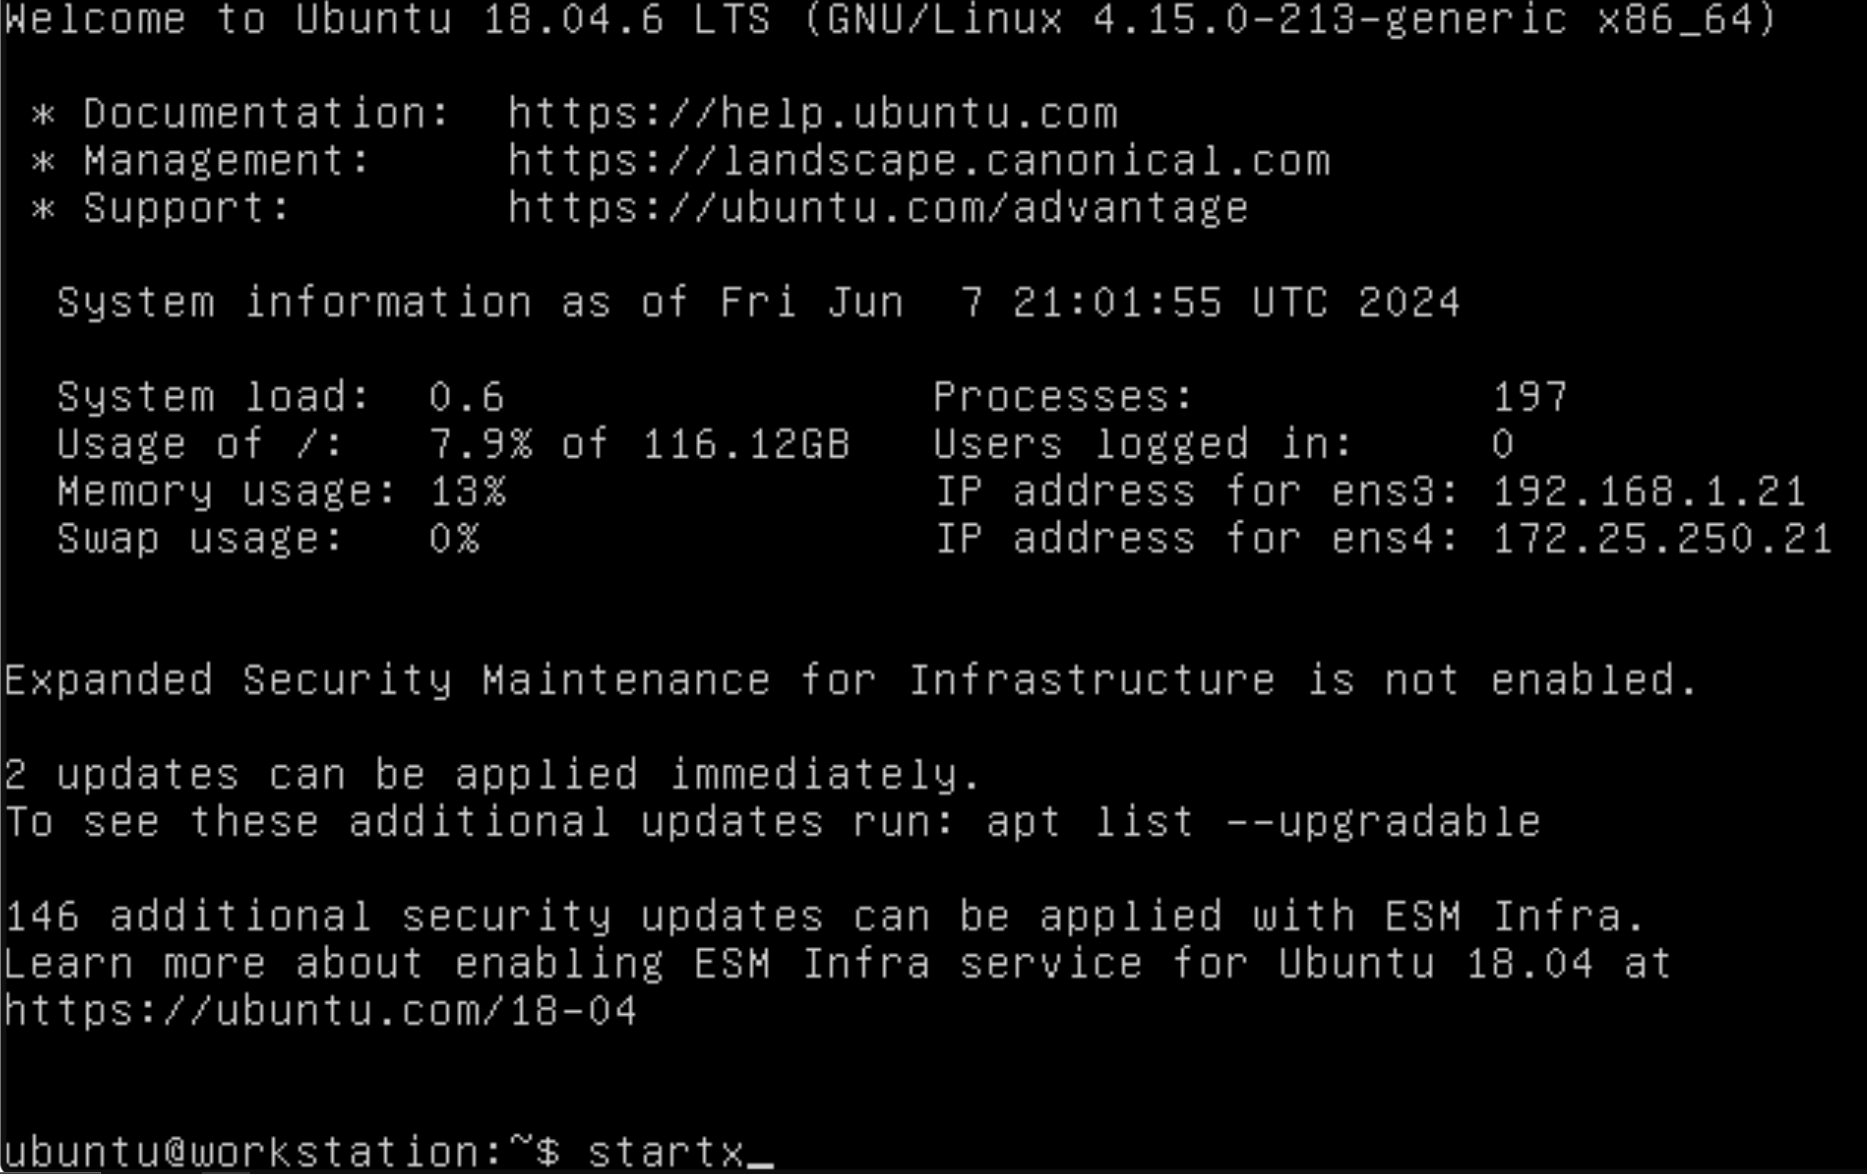
\includegraphics[width=\linewidth]{images/part1/step2.png}
    \end{center}

    \item Click \textbf{Create Image} to create a new image.

    \begin{center}
        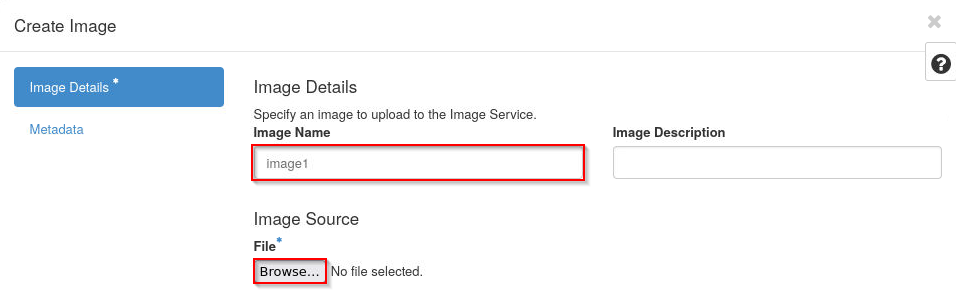
\includegraphics[width=\linewidth]{images/part1/step3.png}
    \end{center}

    \item Enter \textbf{image1} into the \textit{Image Name} field. Under \textbf{File}, click \textbf{Browse...}.
    
    \begin{center}
        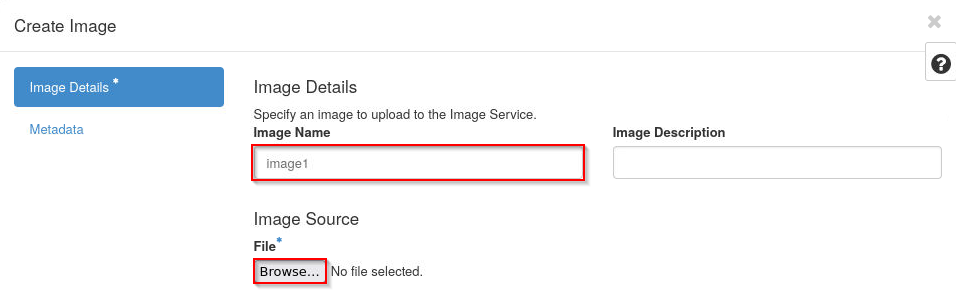
\includegraphics[width=\linewidth]{images/part1/step4.png}
    \end{center}

    \item In the file browser, click \textbf{Downloads}, then select the \textbf{ubuntu.img} file. Click the
    \textbf{Open} button.

    \begin{center}
        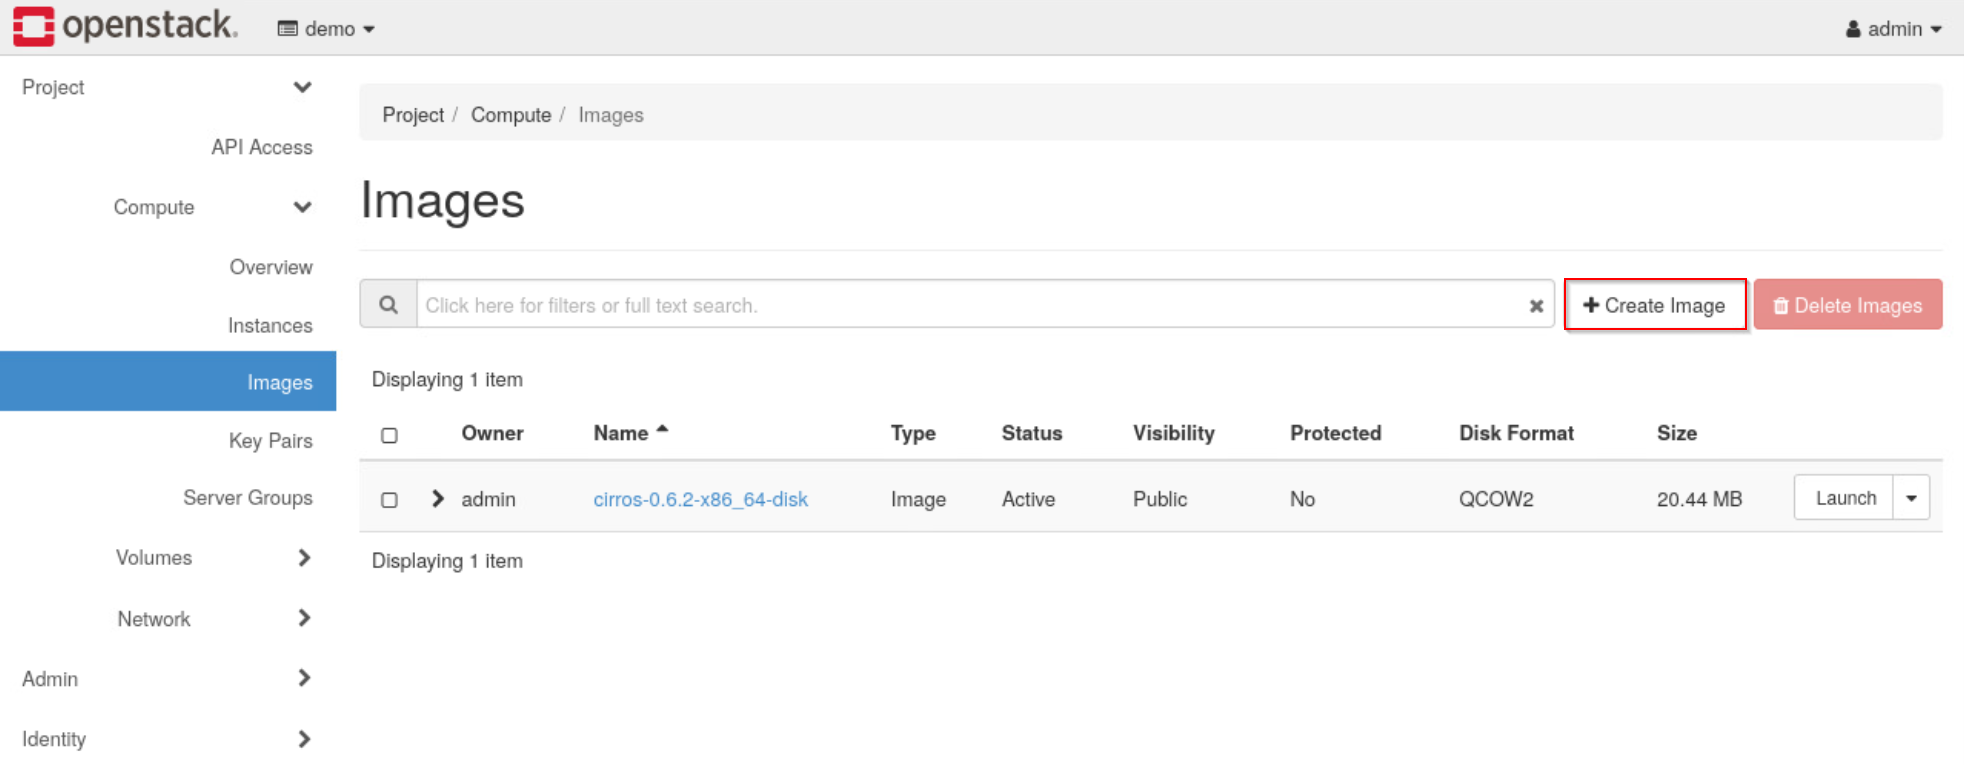
\includegraphics[width=\linewidth]{images/part1/step5.png}
    \end{center}

    \item In the format dropdown, select \textbf{QCOW2 - QEMU Emulator}, and under \textit{Image Sharing}, set
    \textit{Visibility} to \textbf{Private}. Make sure \textbf{No} is selected for \textit{Protected}, and click on
    \textbf{Create Image}.

    \begin{center}
        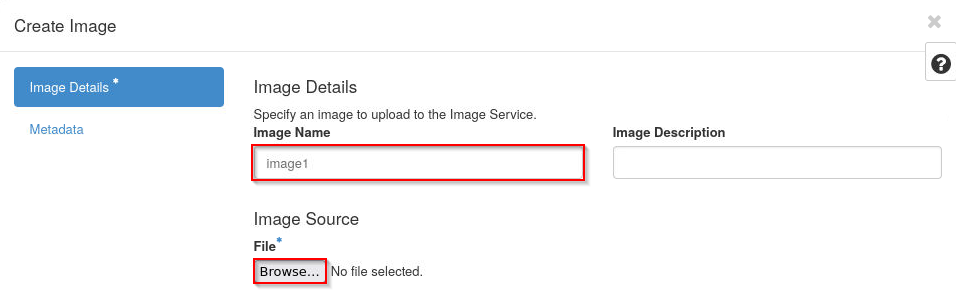
\includegraphics[width=\linewidth]{images/part1/step6.png}
    \end{center}

    \begin{stopbox}{}
        Wait for the \textbf{image1} status to be \textit{Active}. You may need to refresh the browser until you see the
        status of \textit{Active}.
    \end{stopbox}

    \item Open the dropdown menu next to the \textbf{Launch} button in the row of \textbf{image1}, and click on
    \textbf{Edit Image}.

    \begin{center}
        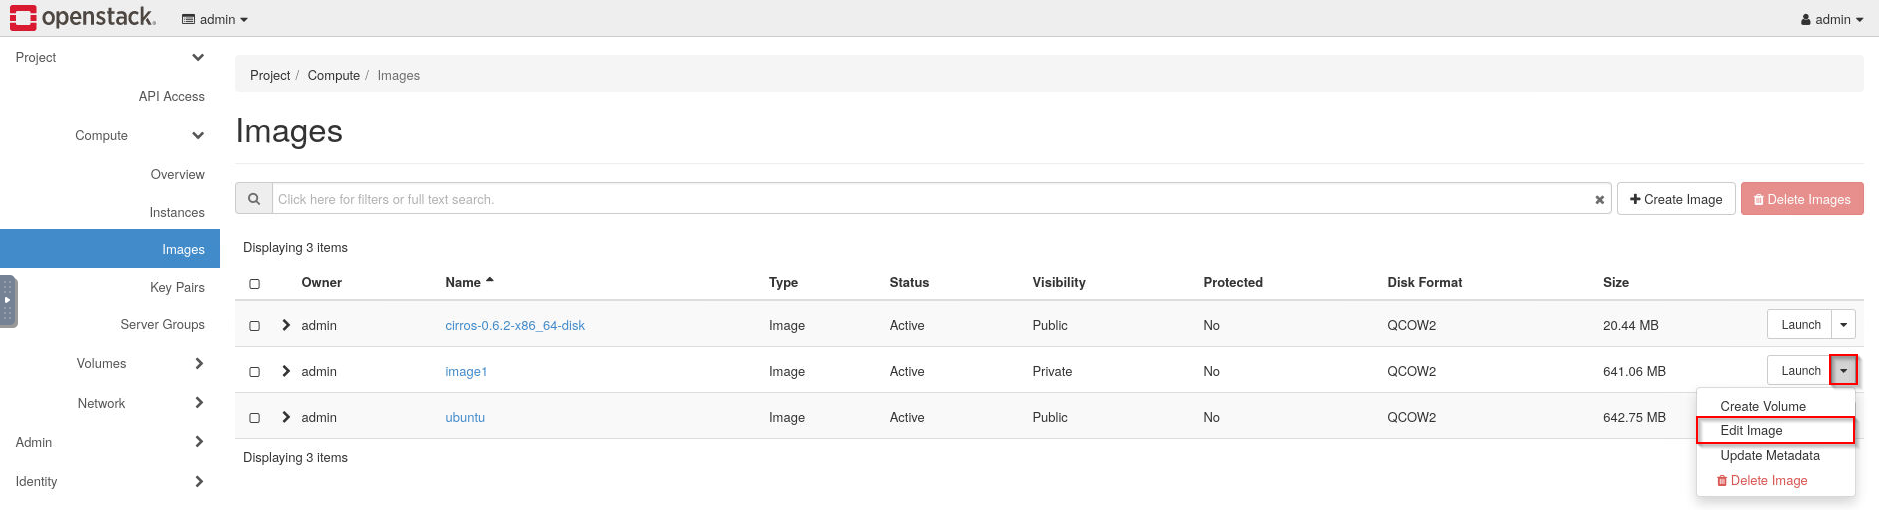
\includegraphics[width=\linewidth]{images/part1/step7.png}
    \end{center}

    \item Enter \textbf{10} in the \textit{Minimum Disk (GB)} field, and select \textbf{Yes} for \textit{Protected}.
    Click the \textbf{Update Image} button.

    \begin{center}
        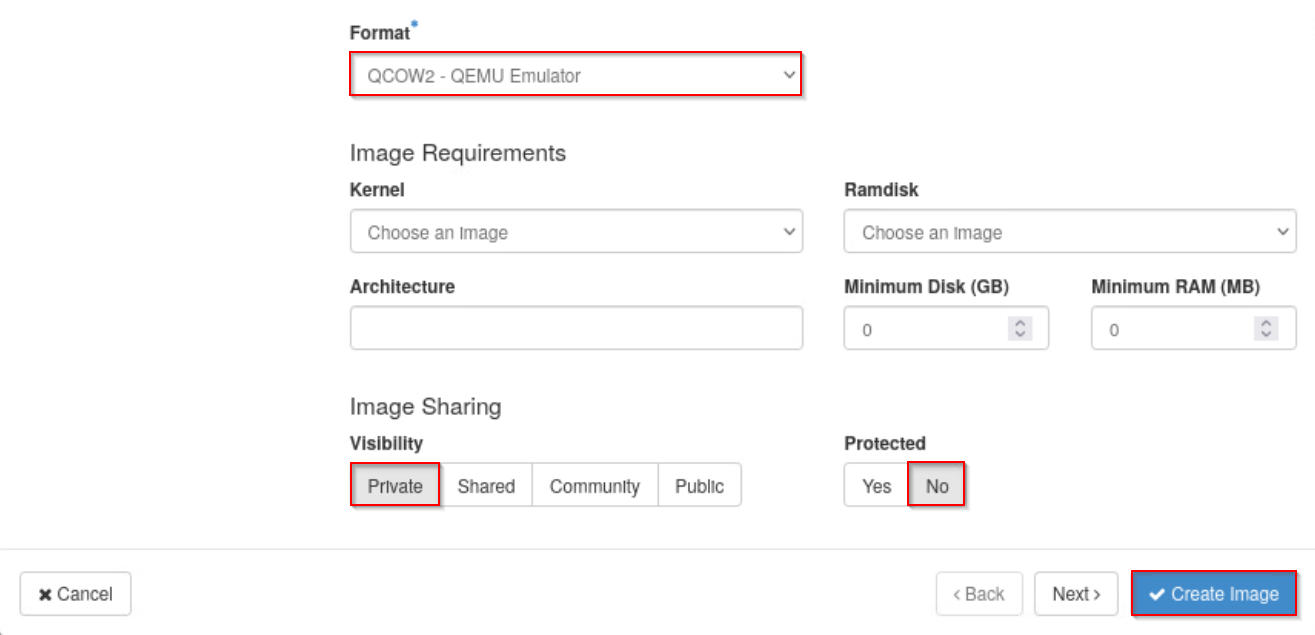
\includegraphics[width=\linewidth]{images/part1/step8.png}
    \end{center}

    \item Log out of the \textit{Horizon Dashboard} and close the web browser.

    \item Open a terminal if one is not already open, and source the \textbf{keystonerc-admin} file to load the
    \textbf{admin} user credentials.
\begin{lstlisting}
ubuntu@workstation:~$ source ~/keystonerc-admin
\end{lstlisting}

    \begin{center}
        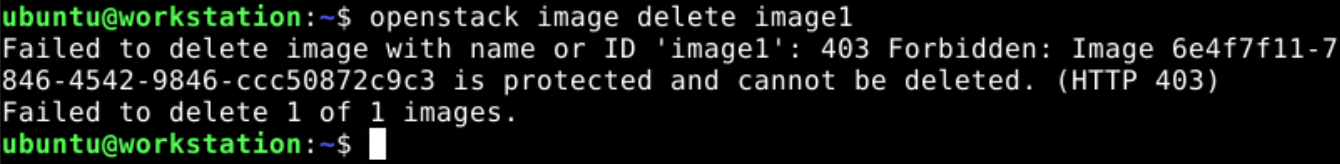
\includegraphics[width=\linewidth]{images/part1/step10.png}
    \end{center}

    \item Try to delete the \textbf{image1} image while it is protected. It should return an error.
\begin{lstlisting}
ubuntu@workstation:~$ openstack image delete image1
\end{lstlisting}

    \begin{center}
        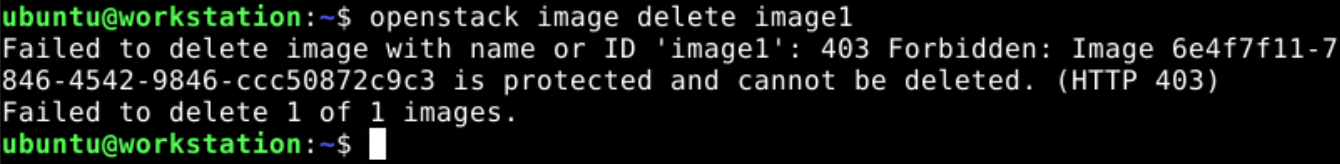
\includegraphics[width=\linewidth]{images/part1/step11.png}
    \end{center}

    \item Set the \textbf{image1} image to unprotected.
\begin{lstlisting}
ubuntu@workstation:~$ openstack image set --unprotected image1
\end{lstlisting}

    \begin{center}
        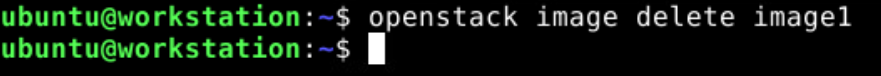
\includegraphics[width=\linewidth]{images/part1/step12.png}
    \end{center}

    \item Delete the \textbf{image1} image.
\begin{lstlisting}
ubuntu@workstation:~$ openstack image delete image1
\end{lstlisting}

    \begin{center}
        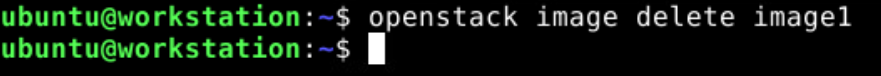
\includegraphics[width=\linewidth]{images/part1/step13.png}
    \end{center}

    \item Create the \textbf{image1} image using the \textbf{\texttildemid/Downloads/ubuntu.img} file and the QCOW2
    format.
\begin{lstlisting}
ubuntu@workstation:~$ openstack image create \
> --disk-format qcow2 \
> --file ~/Downloads/ubuntu.img \
> image2
\end{lstlisting}

    \begin{center}
        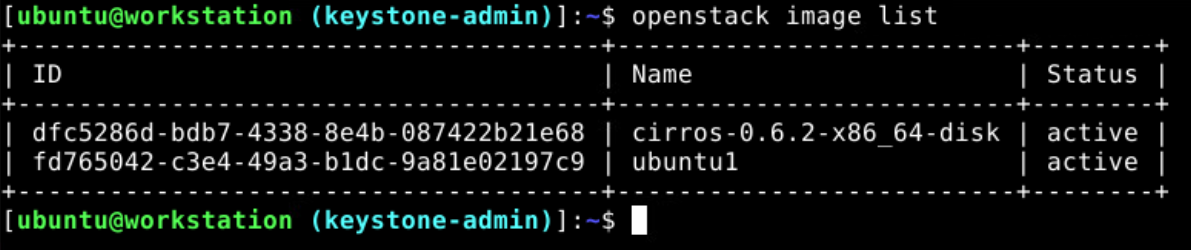
\includegraphics[width=\linewidth]{images/part1/step14.png}
    \end{center}

    \item Set the \textbf{image2} image status to \textbf{protected}, and set the minimum disk size to \textbf{10 GB}.
\begin{lstlisting}
ubuntu@workstation:~$ openstack image set \
> --protected \
> --min-disk 10 \
> image2
\end{lstlisting}

    \begin{center}
        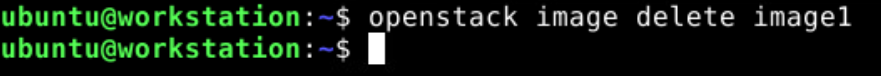
\includegraphics[width=\linewidth]{images/part1/step15.png}
    \end{center}

    \item Set the \textbf{image2} image to be public. Note that this action requires administrative privileges.
\begin{lstlisting}
ubuntu@workstation:~$ openstack image set --public image2
\end{lstlisting}

    \begin{center}
        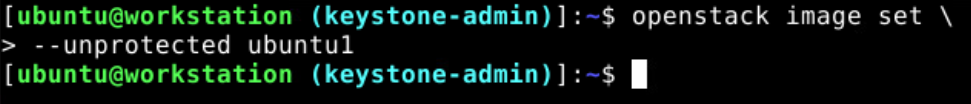
\includegraphics[width=\linewidth]{images/part1/step16.png}
    \end{center}

    \item Verify that the \textbf{image2} image was correctly created by listing the available images.
\begin{lstlisting}
ubuntu@workstation:~$ openstack image list
\end{lstlisting}

    \begin{center}
        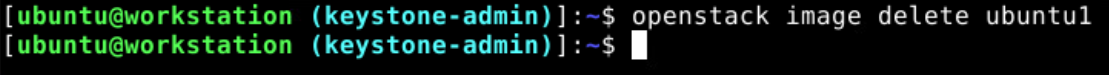
\includegraphics[width=\linewidth]{images/part1/step17.png}
    \end{center}

    \item Display the details of the \textbf{image2} image and verify that it was correctly updated. Confirm the value
    for the \textit{min\_disk} field is \textbf{10}, the value for the \textit{protected} field is \textbf{True}, and
    the value for \textit{visibility} is \textbf{public}.
\begin{lstlisting}
ubuntu@workstation:~$ openstack image show image2
\end{lstlisting}

    \begin{center}
        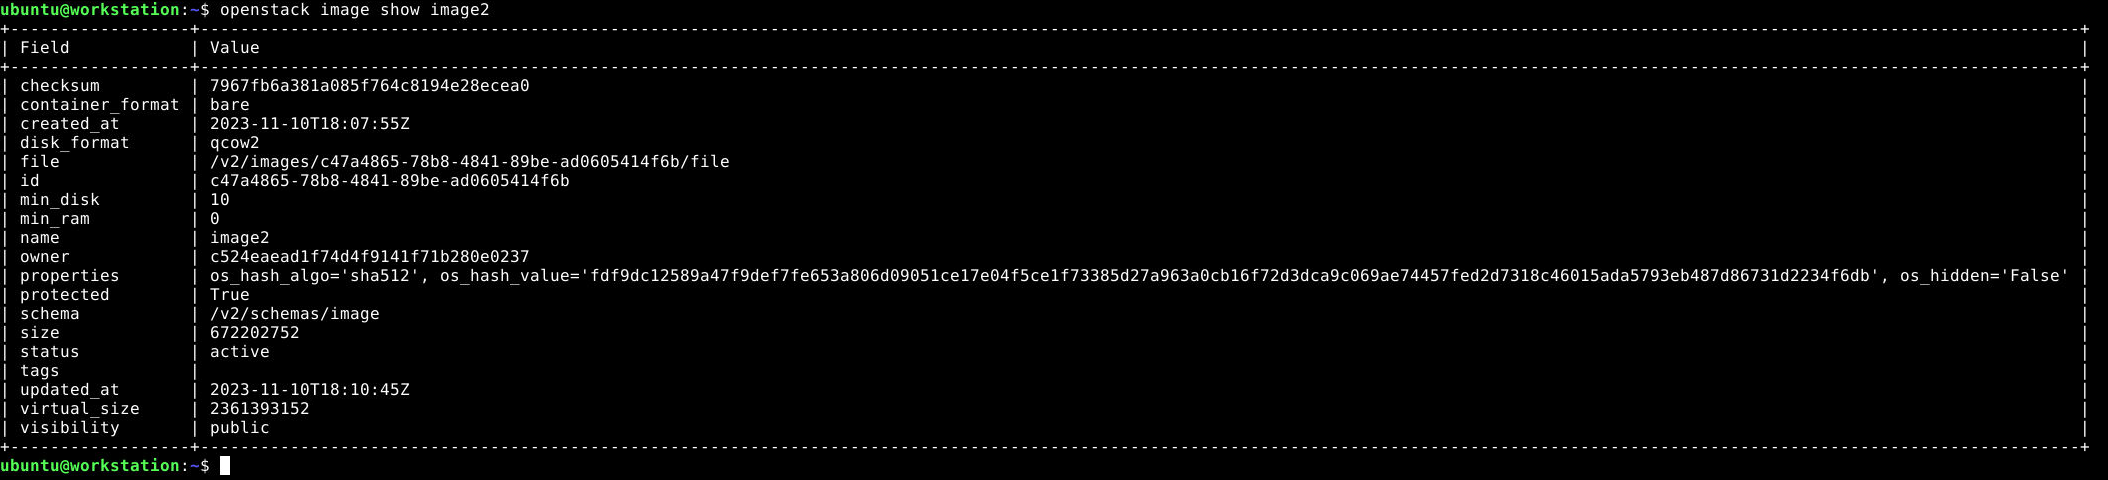
\includegraphics[width=\linewidth]{images/part1/step18.png}
    \end{center}

    \item Leave the terminal window open and continue to the next task.

\end{enumerate}

\section{Developing Flavors}
\label{sec:developing_flavors}
In this task, you will create, modify, and delete flavors using the \textit{Horizon Dashboard} and
\textit{OpenStack Unified CLI}.

\begin{enumerate}
    \item Open the web browser and navigate to \textbf{192.168.1.20}. Log in to the dashboard as the \textbf{admin} user
    with the password \textbf{secret}.
    
    \item Switch to the \textbf{demo} project. Navigate to \textbf{Admin $>$ Compute $>$ Flavors} and click
    \textbf{Create Flavor}.

    \begin{center}
        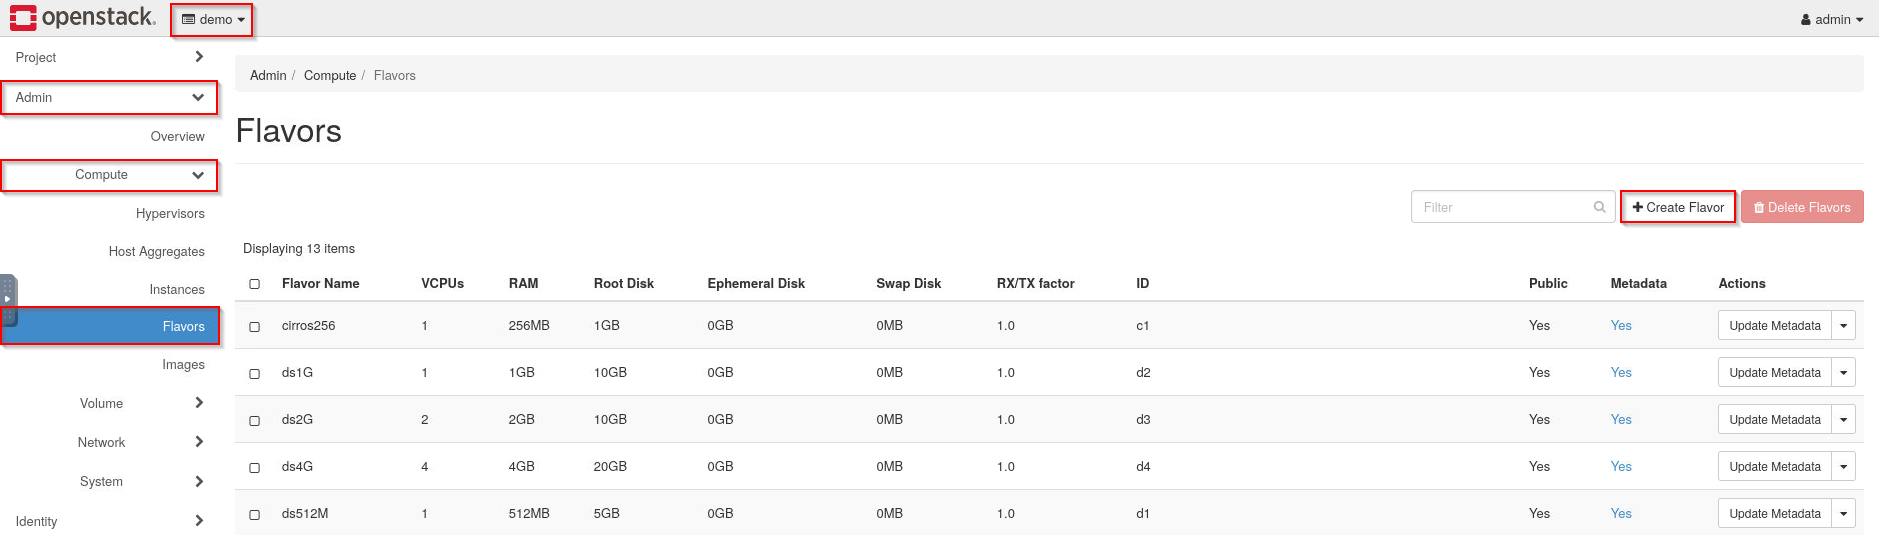
\includegraphics[width=\linewidth]{images/part2/step2.png}
    \end{center}

    \item Enter \textbf{flavor1} in the \textit{Name} field, \textbf{2} in the \textit{VCPUs} field, \textbf{1024} in
    the \textit{RAM (MB)} field, and \textbf{10} in the \textit{Root Disk (GB)} field. Click on \textbf{Create Flavor}.

    \begin{center}
        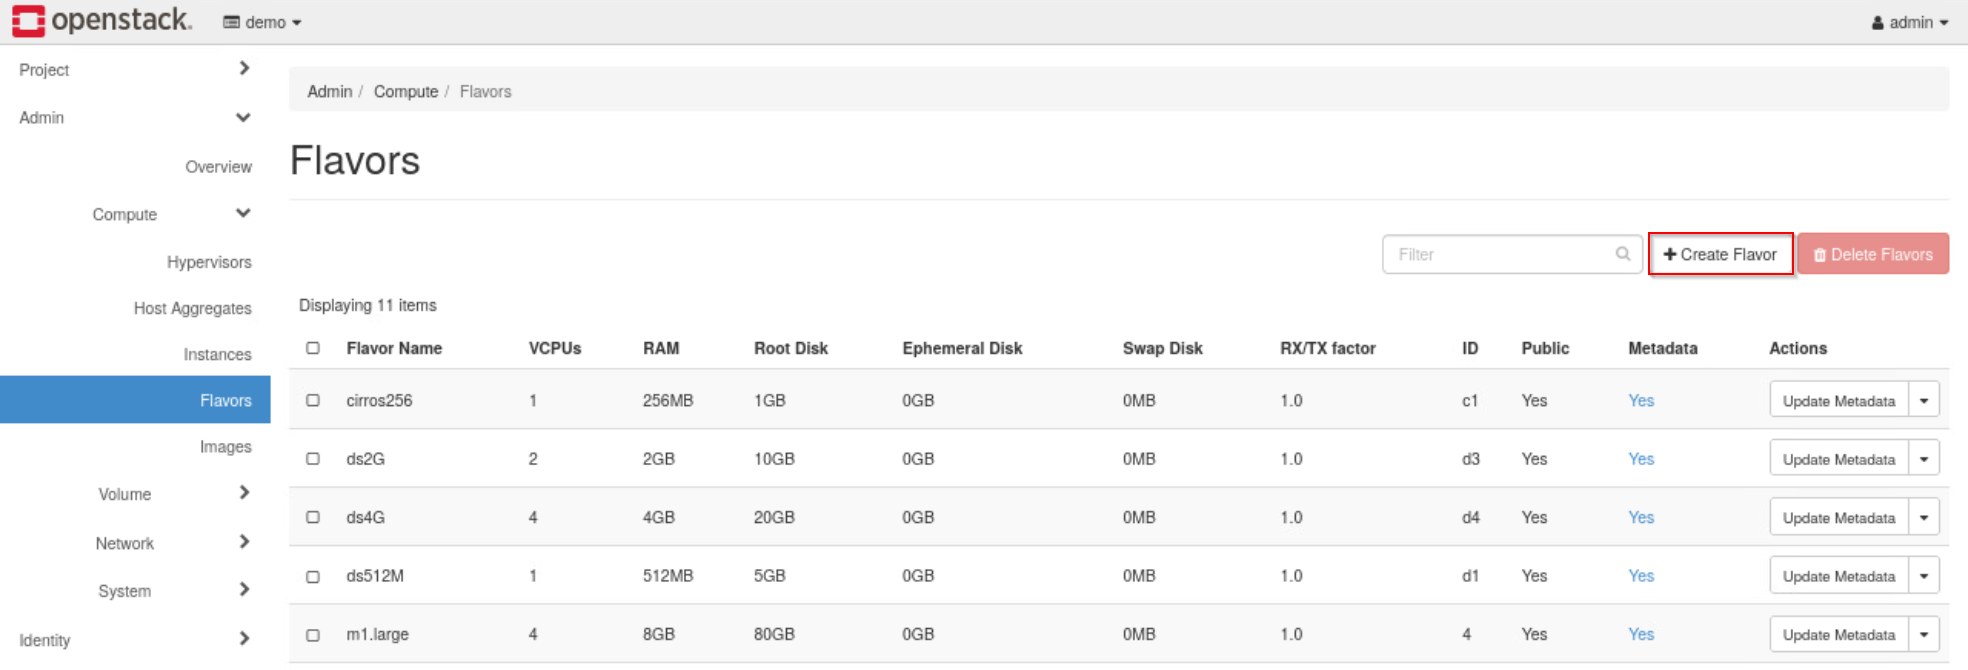
\includegraphics[width=\linewidth]{images/part2/step3.png}
    \end{center}

    \item Log out of the \textit{Horizon Dashboard} and close the web browser.
    
    \item If a terminal is not already open, open one and source the \textbf{\texttildemid/keystonerc-admin} file.

    \item Create a flavor named \textbf{m1.exercise}. Configure the flavor with \textbf{1} VCPU, \textbf{1024 MB} of RAM, a
    \textbf{10 GB} root disk, a \textbf{2 GB} ephemeral disk, and a \textbf{1024 MB} swap disk.
\begin{lstlisting}
ubuntu@workstation:~$ openstack flavor create \
> --vcpus 1 \
> --ram 1024 \
> --disk 10 \
> --ephemeral 2 \
> --swap 1024 \
> m1.exercise
\end{lstlisting}

    \begin{center}
        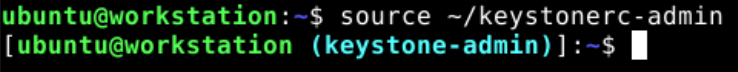
\includegraphics[width=\linewidth]{images/part2/step6.png}
    \end{center}

    \item Verify that the \textbf{m1.exercise} flavor has been created with the correct settings.
\begin{lstlisting}
ubuntu@workstation:~$ openstack flavor show m1.exercise
\end{lstlisting}

    \begin{center}
        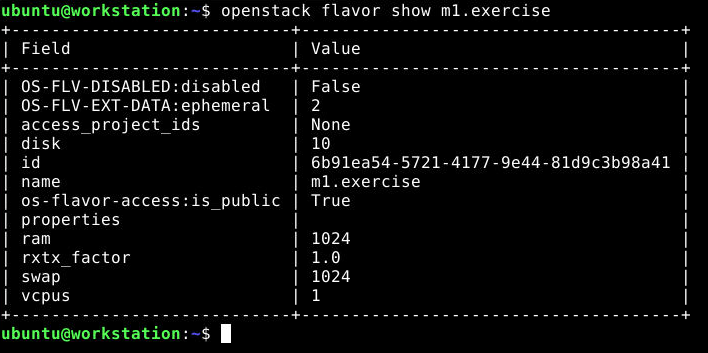
\includegraphics[width=\linewidth]{images/part2/step7.png}
    \end{center}

    \item Delete the \textbf{flavor1} flavor.
\begin{lstlisting}
ubuntu@workstation:~$ openstack flavor delete flavor1
\end{lstlisting}

    \begin{center}
        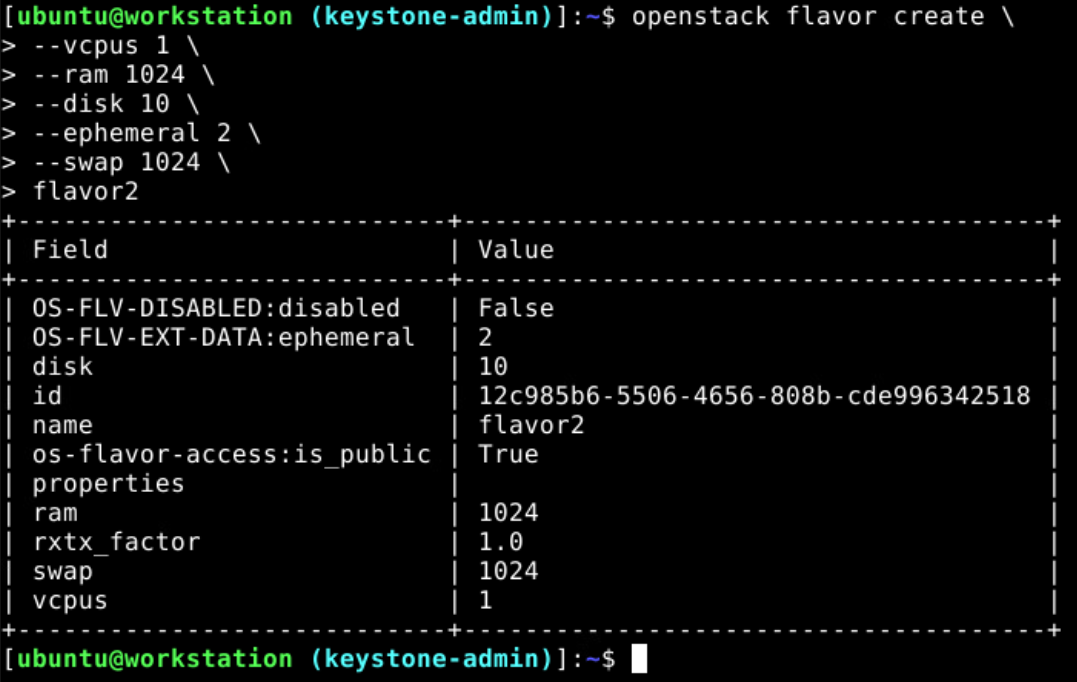
\includegraphics[width=\linewidth]{images/part2/step8.png}
    \end{center}

    \item Verify that the \textbf{flavor1} has been deleted by listing all the available flavors and noting that
    \textbf{flavor1} does not appear in the list.
\begin{lstlisting}
ubuntu@workstation:~$ openstack flavor list    
\end{lstlisting}

    \begin{center}
        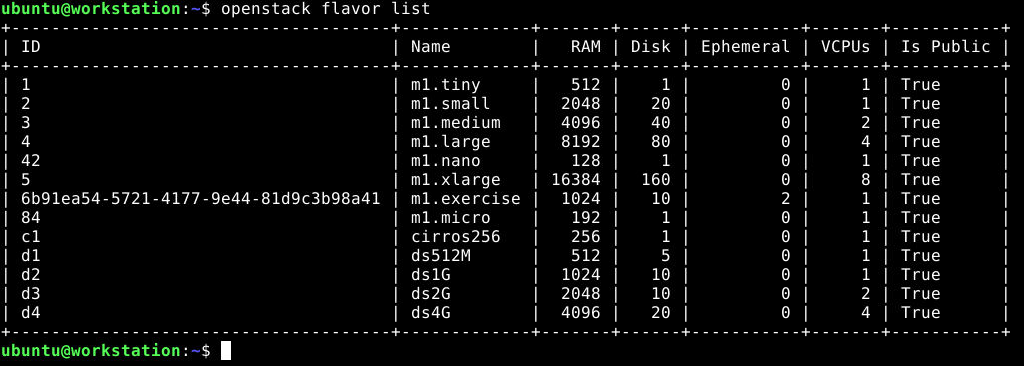
\includegraphics[width=\linewidth]{images/part2/step9.png}
    \end{center}

    \begin{tipbox}{}
        An alternative method is appending \textbf{\texttt{| grep flavor1}} to this command and noting that there is no
        output.
    \end{tipbox}

    \item Leave the terminal window open and continue to the next task.
\end{enumerate}

\section{Managing Private Networks}
\label{sec:managing_private_networks}
In this task, you will manage networks and subnets using the \textit{Horizon Dashboard} and \textit{OpenStack
Unified CLI}. You will create and delete networks and subnetworks, update their settings, and rename them.

\begin{enumerate}
    \item Open the web browser and navigate to \textbf{192.168.1.20}. Log in to the dashboard as the \textbf{admin} user
    with the password \textbf{secret}.

    \item Navigate to \textbf{Project $>$ Network $>$ Networks} and click \textbf{Create Network}.

    \begin{center}
        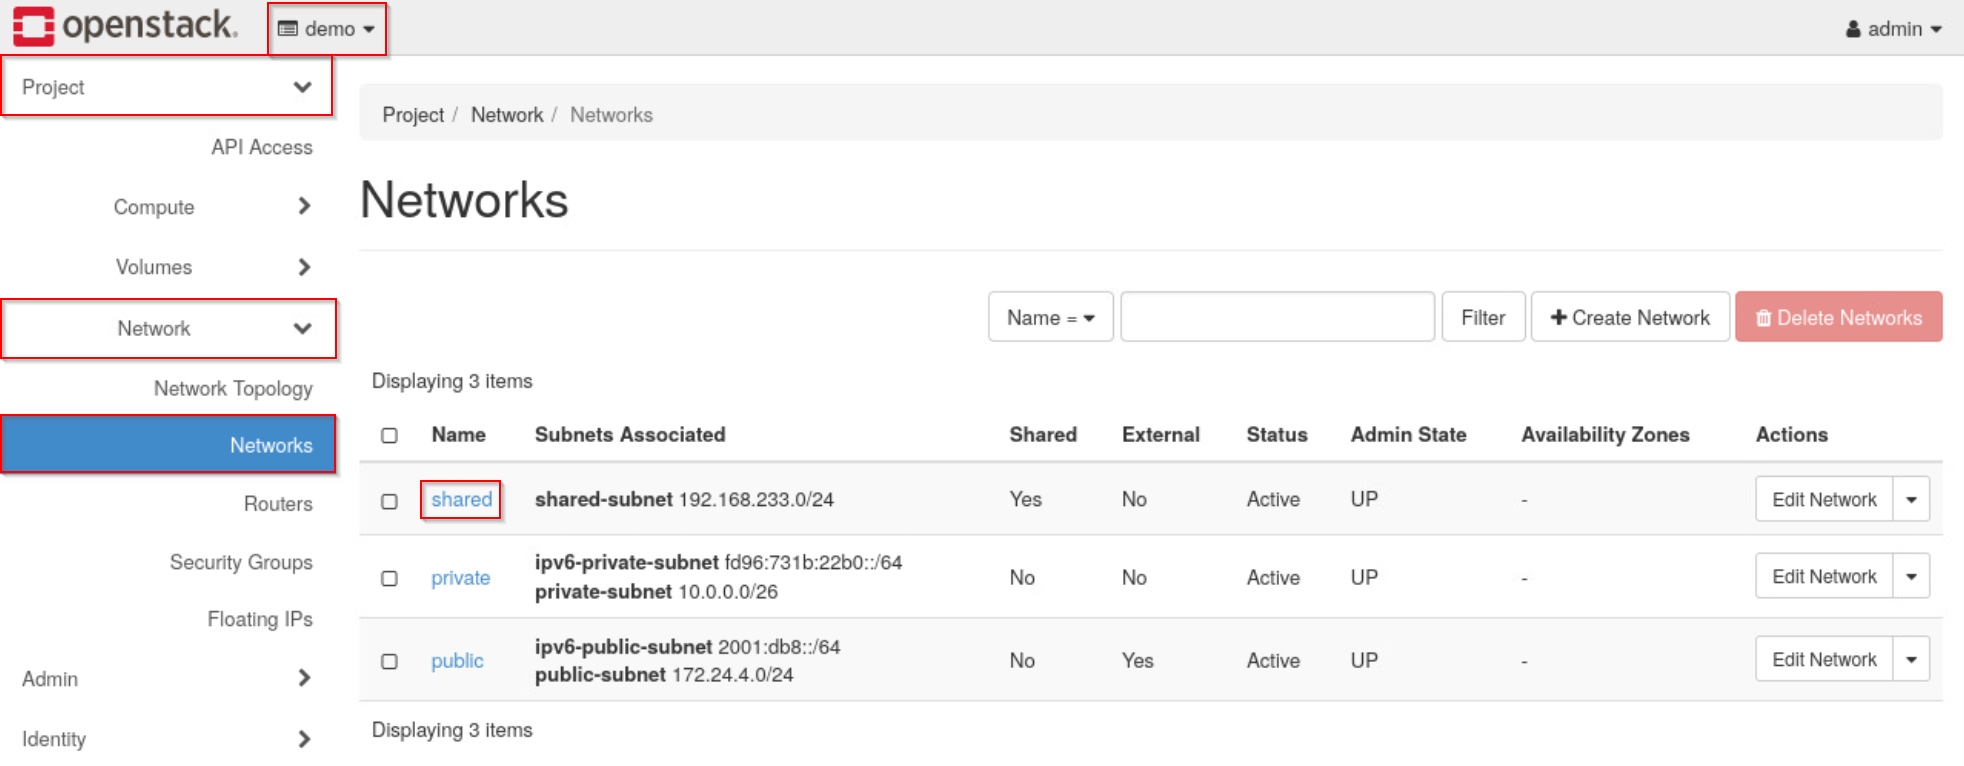
\includegraphics[width=\linewidth]{images/part3/step2.png}
    \end{center}

    \item Enter \textbf{net1} in the \textit{Network Name} field. Verify that the \textbf{Create Subnet} check box is
    selected. Click \textbf{Next}.

    \begin{center}
        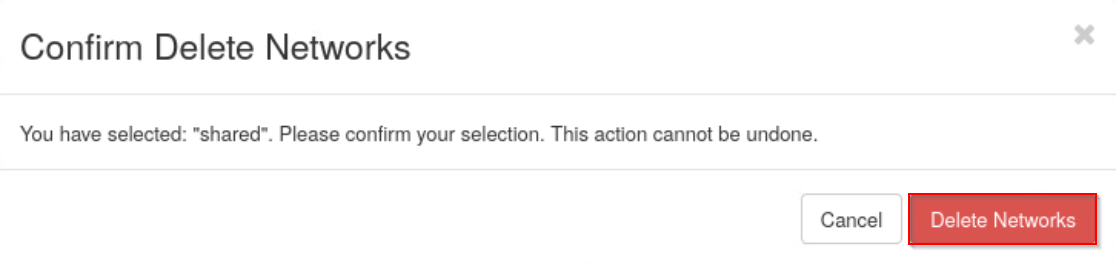
\includegraphics[width=\linewidth]{images/part3/step3.png}
    \end{center}

    \item Enter \textbf{subnet1} in the \textit{Subnet Name} field, and enter \textbf{10.0.0.0/24} in the
    \textit{Network Address} field. Click \textbf{Next}.

    \begin{center}
        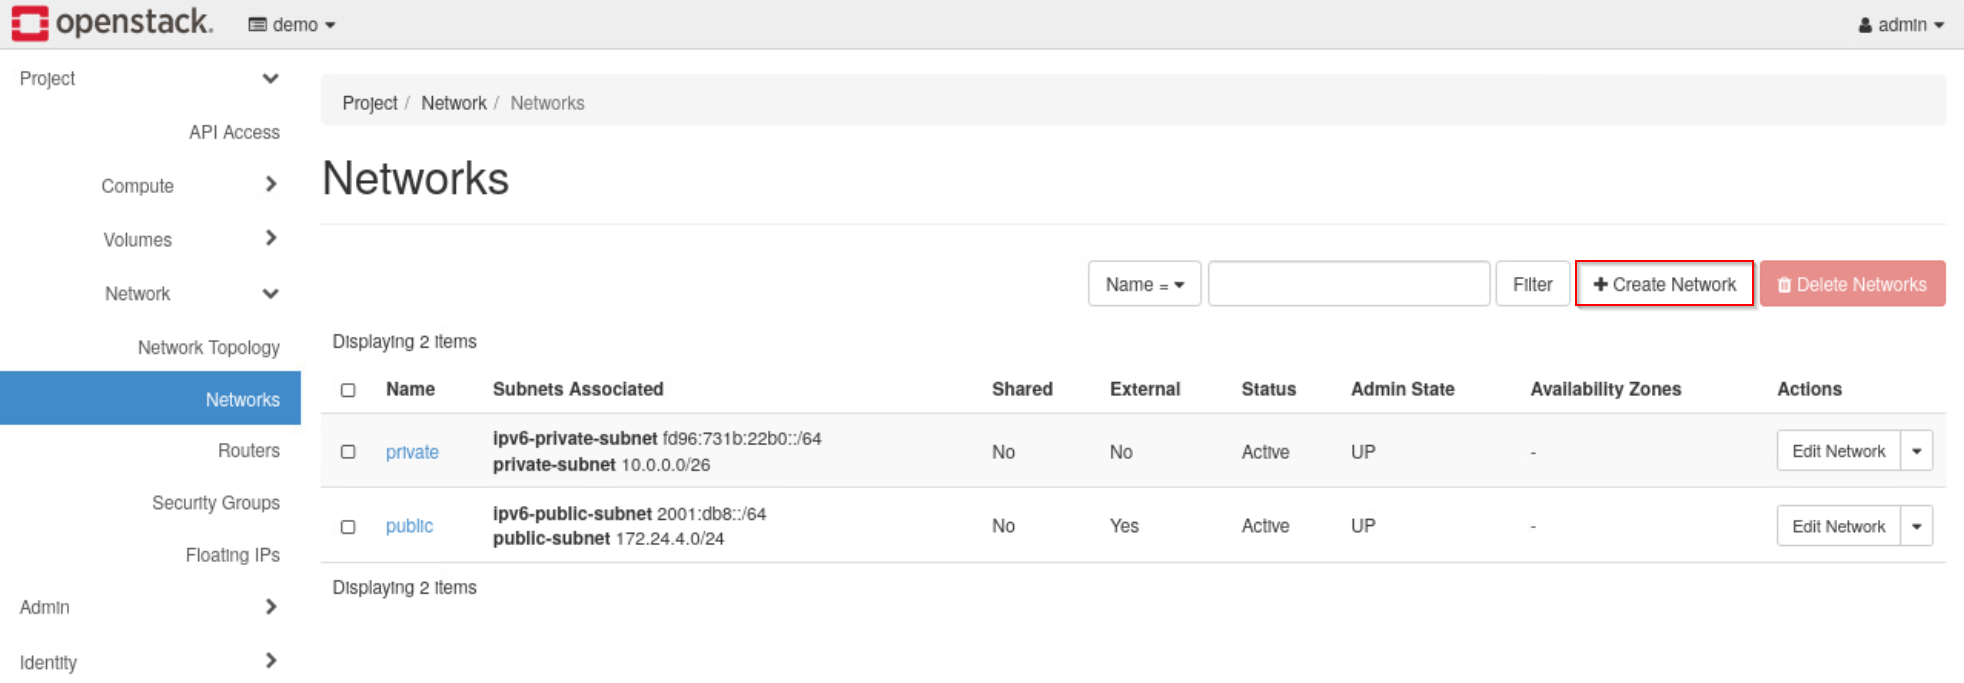
\includegraphics[width=\linewidth]{images/part3/step4.png}
    \end{center}

    \item Leave the defaults in the \textit{Subnet Details} tab and click \textbf{Create}.
    
    \begin{center}
        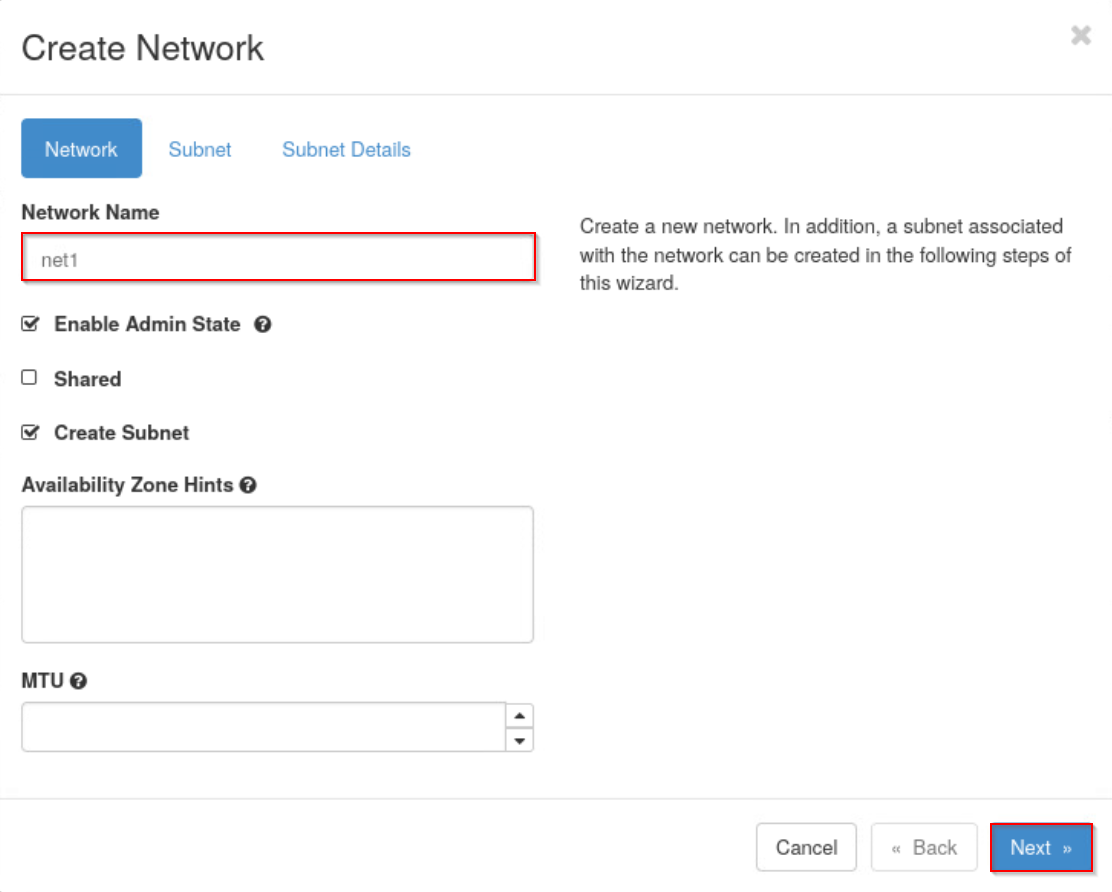
\includegraphics[width=\linewidth]{images/part3/step5.png}
    \end{center}

    \item Log out of the \textit{Horizon Dashboard} and close the web browser.
    
    \item If a terminal window is not already open, open one and source the \textbf{\texttildemid/keystonerc-admin} file
    to load the \textbf{admin} user credentials.
    
    \item Create a network named \textbf{exercise} using the command below.
\begin{lstlisting}
ubuntu@workstation:~$ openstack network create exercise
\end{lstlisting}

    \begin{center}
        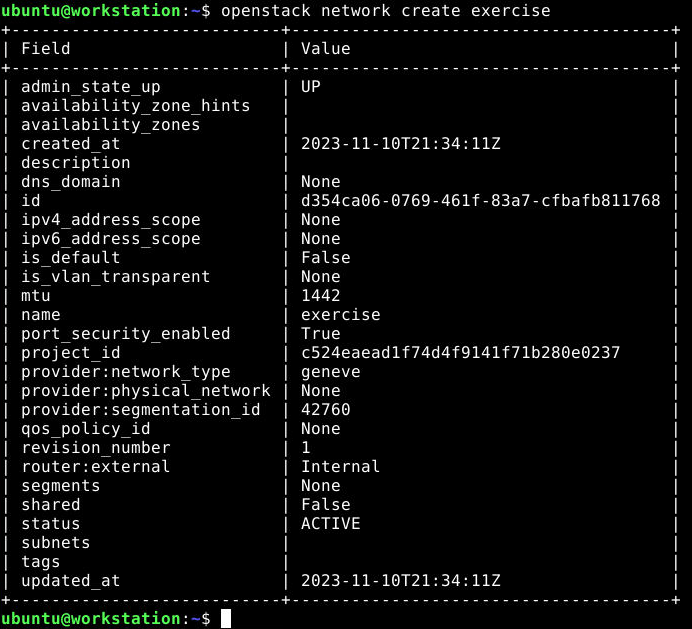
\includegraphics[width=\linewidth]{images/part3/step8.png}
    \end{center}

    \item Create a subnet named \textbf{subexer} for the \textbf{exercise} network. Configure this subnet to use the
    \textbf{192.168.1.0./24} range and \textbf{172.25.250.254} as the DNS name server.
\begin{lstlisting}
ubuntu@workstation:~$ openstack subnet create \
> --subnet-range 192.168.1.0/24 \
> --dns-nameserver 172.25.250.254 \
> --network exercise \
> subexer
\end{lstlisting}

    \begin{center}
        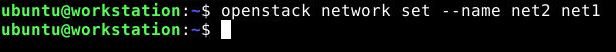
\includegraphics[width=\linewidth]{images/part3/step9.png}
    \end{center}

    \item Change the name of the \textbf{net1} network to \textbf{net2}.
\begin{lstlisting}
ubuntu@workstation:~$ openstack network set --name net2 net1
\end{lstlisting}

    \begin{center}
        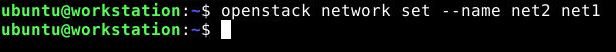
\includegraphics[width=\linewidth]{images/part3/step10.png}
    \end{center}

    \begin{notebox}{}
        The desired name for the network follows the \textbf{\texttt{--name}} option, while the current network name is
        the final argument of the command.
    \end{notebox}

    \item Verify that the \textbf{net1} network has been successfully changed to \textbf{net2}.
\begin{lstlisting}
ubuntu@workstation:~$ openstack network list
\end{lstlisting}

    \begin{center}
        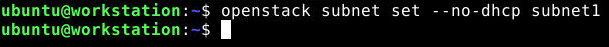
\includegraphics[width=\linewidth]{images/part3/step11.png}
    \end{center}

    \item Update the \textbf{subnet1} subnetwork to disable DHCP.
\begin{lstlisting}
ubuntu@workstation:~$ openstack subnet set --no-dhcp subnet1
\end{lstlisting}

    \begin{center}
        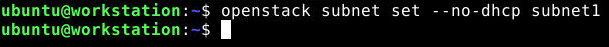
\includegraphics[width=\linewidth]{images/part3/step12.png}
    \end{center}

    \item Verify that the \textbf{subnet1} subnetwork has been correctly updated.
\begin{lstlisting}
ubuntu@workstation:~$ openstack subnet show subnet1
\end{lstlisting}

    \begin{center}
        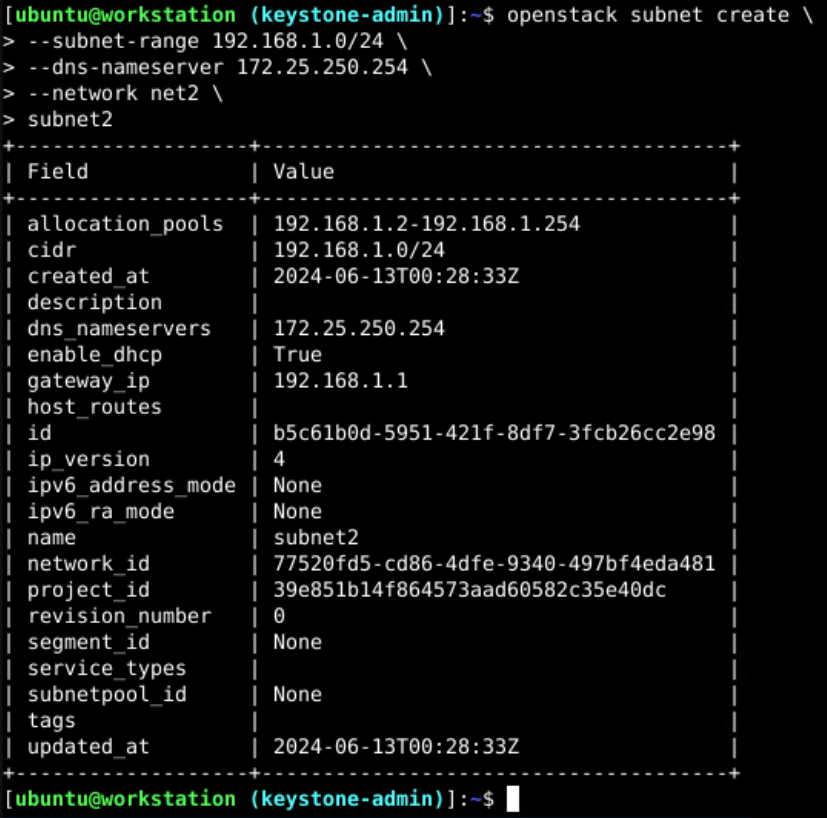
\includegraphics[width=\linewidth]{images/part3/step13.png}
    \end{center}

    \item Delete the \textbf{net2} network.
\begin{lstlisting}
ubuntu@workstation:~$ openstack network delete net2
\end{lstlisting}

    \begin{center}
        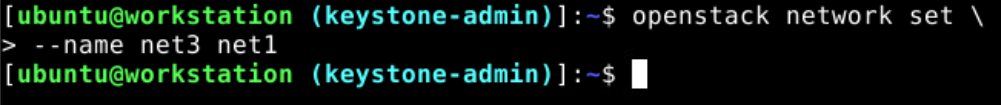
\includegraphics[width=\linewidth]{images/part3/step14.png}
    \end{center}

    \item Verify that the \textbf{net2} network has been deleted by listing all available networks and noting that
    \textbf{net2} is not present in the list.
\begin{lstlisting}
ubuntu@workstation:~$ openstack network list
\end{lstlisting}

    \begin{center}
        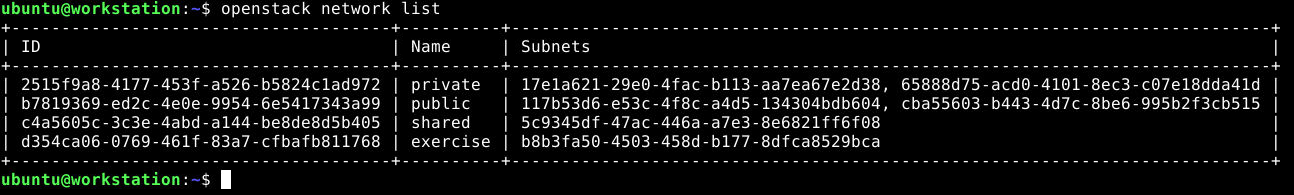
\includegraphics[width=\linewidth]{images/part3/step15.png}
    \end{center}

    \item Leave the terminal window open and continue to the next task.

\end{enumerate}

\section{Launching an Internal Instance}
\label{sec:launching_an_internal_instance}
In this task, you will launch an internal instance with the \textit{Horizon Dashboard}. You will then delete that
instance and launch a new instance by using the \textit{Horizon Unified CLI}.

\begin{enumerate}
    \item Open the web browser and navigate to \textbf{192.168.1.20}. Login as the \textbf{admin} user with the password
    \textbf{secret}.

    \item Switch to the \textbf{demo} project and navigate to
    \textbf{Projects $>$ Compute $>$ Instances}. Click \textbf{Launch Instance}.

    \begin{center}
        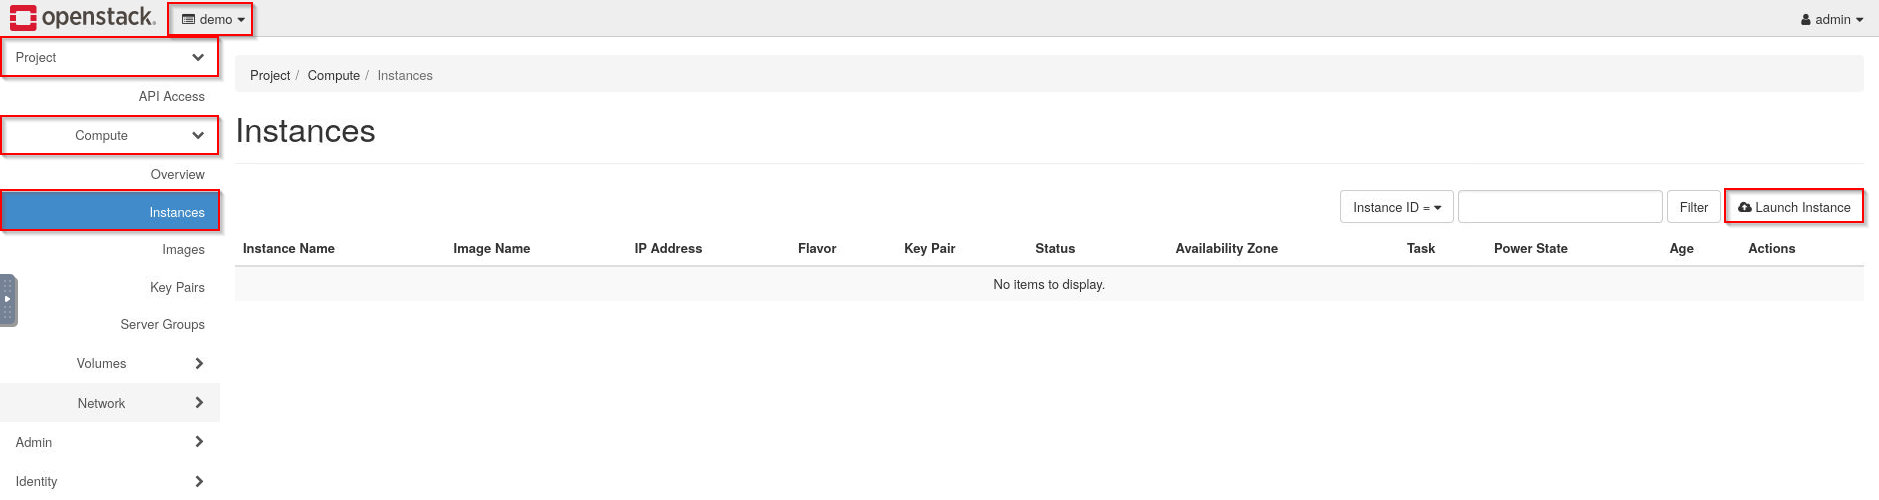
\includegraphics[width=\linewidth]{images/part4/step2.png}
    \end{center}

    \item Ensure that \textbf{demo} is entered in the \textit{Project Name} field, and enter \textbf{instance1} in the
    \textit{Instance Name} field. Click \textbf{Next}.
    
    \begin{center}
        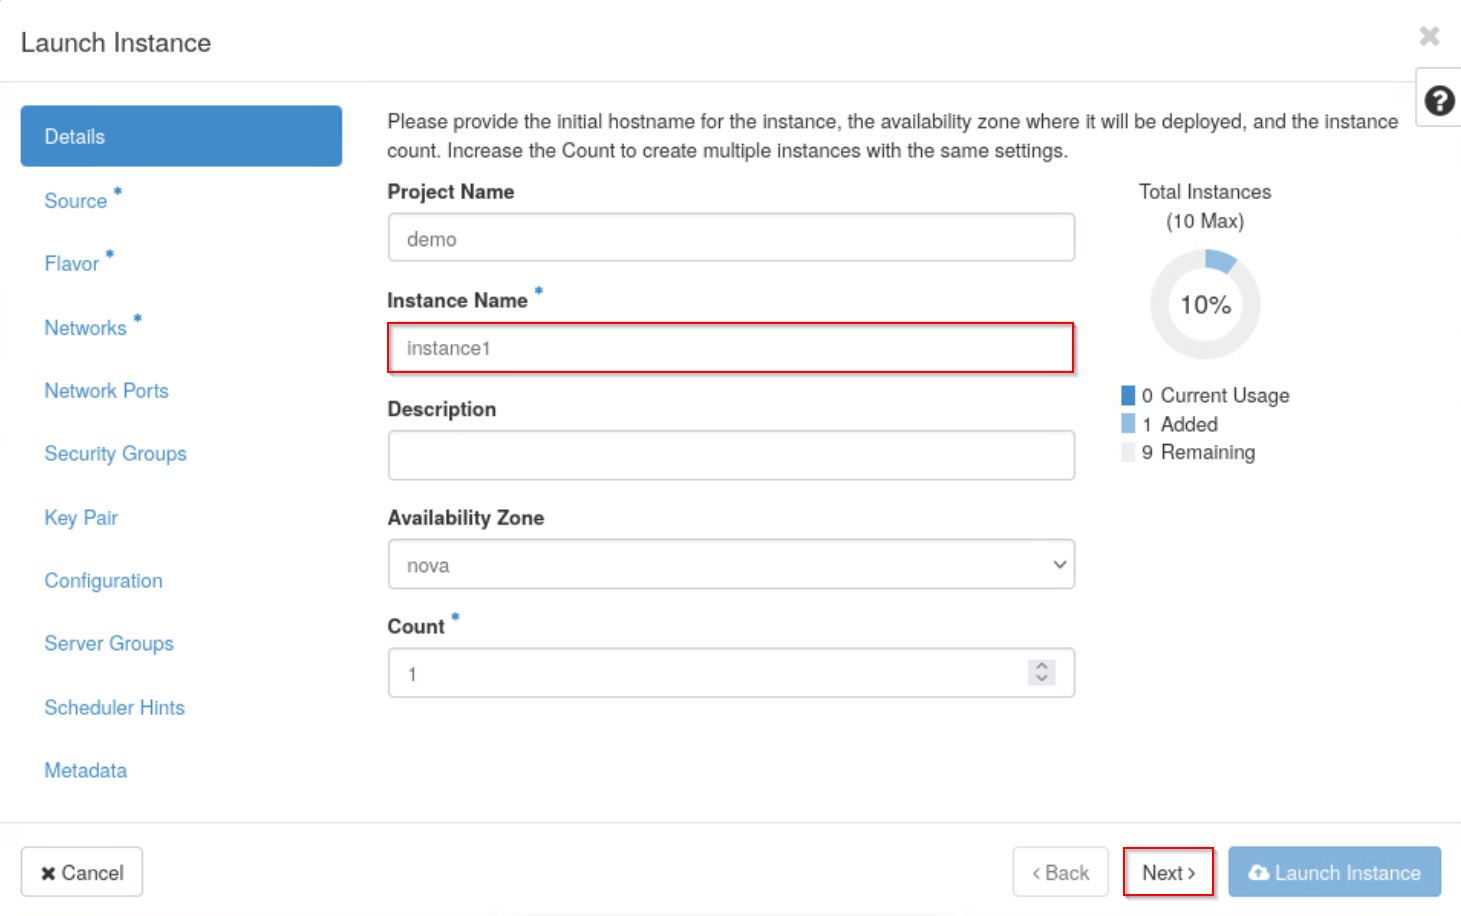
\includegraphics[width=\linewidth]{images/part4/step3.png}
    \end{center}

    \item Make sure \textbf{Image} is selected in the \textit{Select Boot Source} dropdown, and click \textbf{No} under
    \textit{Create New Volume}. Click the $\uparrow$ button on the same row as the \textbf{image2} image to allocate the
    image, and then click \textbf{Next}.

    \begin{center}
        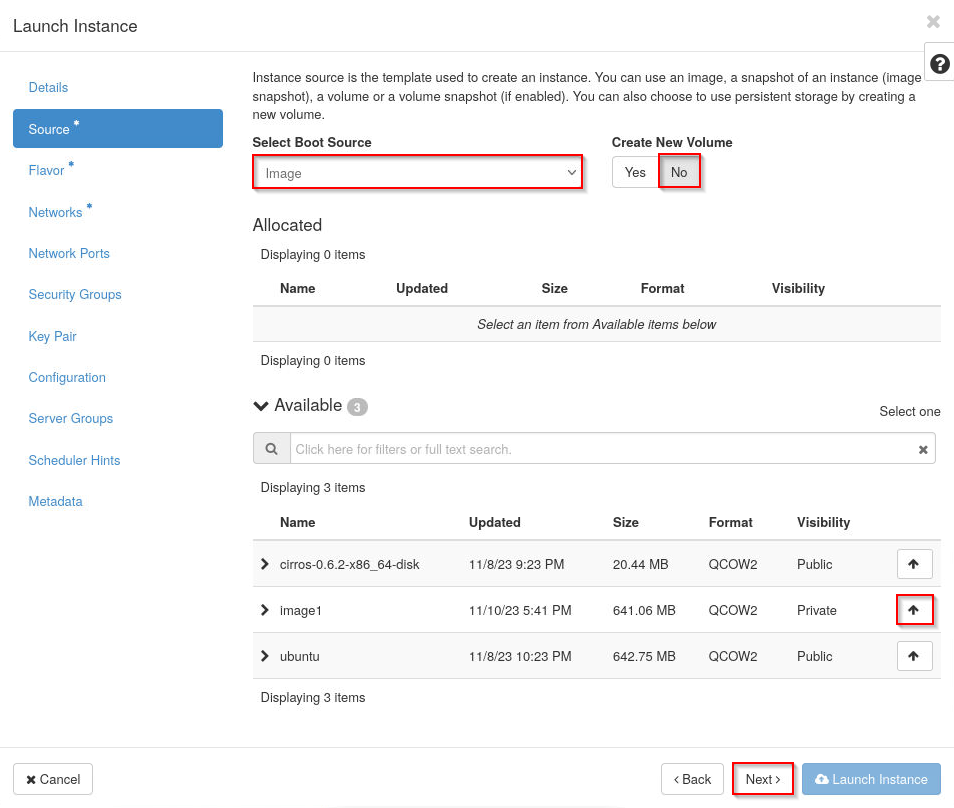
\includegraphics[width=\linewidth]{images/part4/step4.png}
    \end{center}

    \begin{stopbox}{}
        Verify that \textbf{image2} appears in the \textit{Allocated} section before moving on to the next step.
    \end{stopbox}

    \item Click the $\uparrow$ button on the same row as the \textbf{m1.exercise} flavor to allocate that flavor, then
    click \textbf{Next}.
    \begin{center}
        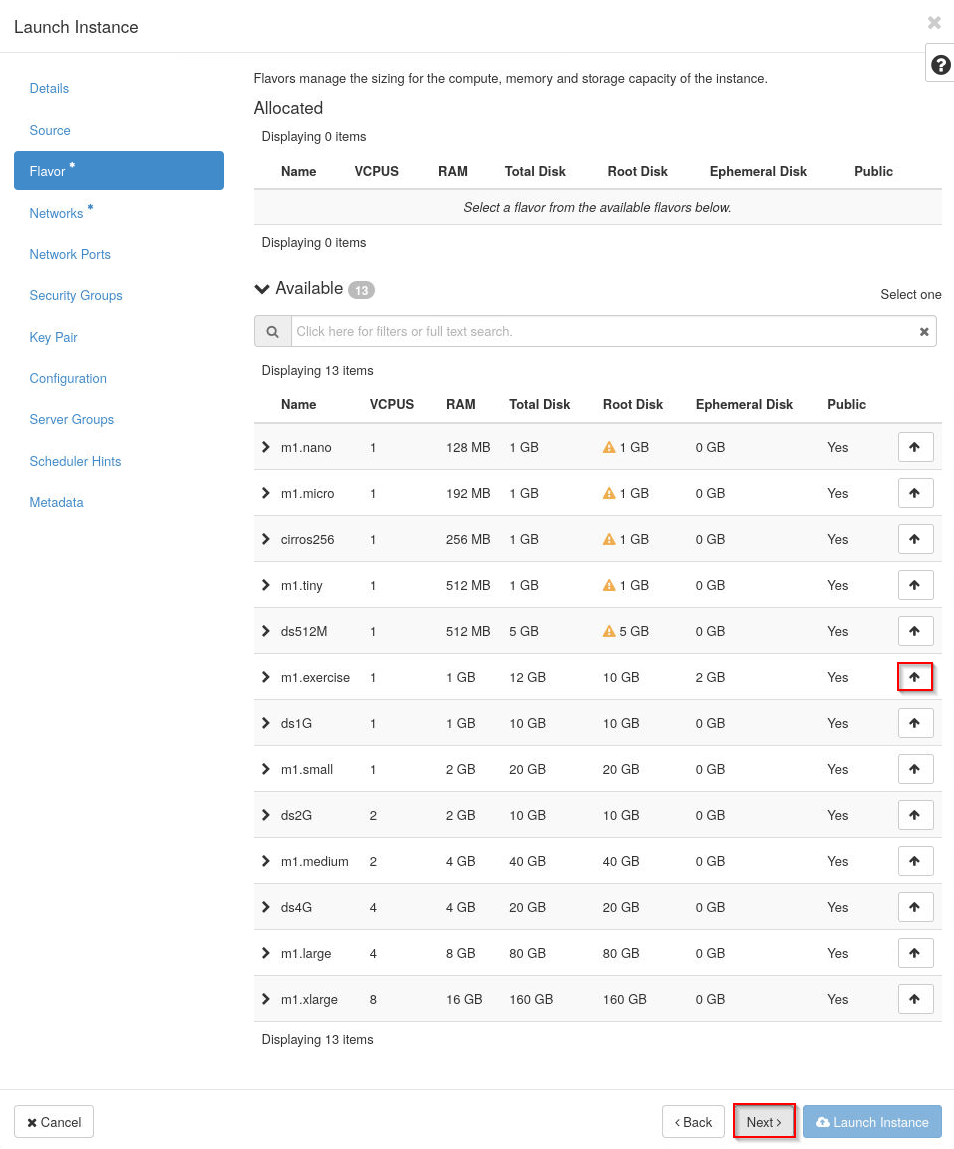
\includegraphics[width=\linewidth]{images/part4/step5.png}
    \end{center}

    \begin{notebox}{}
        The warning signs in the \textit{Root Disk} column indicate that the flavor in that row has a disk size less
        than the minimum size specified for the selected image.
    \end{notebox}

    \item Click the $\uparrow$ button on the same row as the \textbf{exercise} network, and click \textbf{Launch
    Instance}.

    \begin{center}
        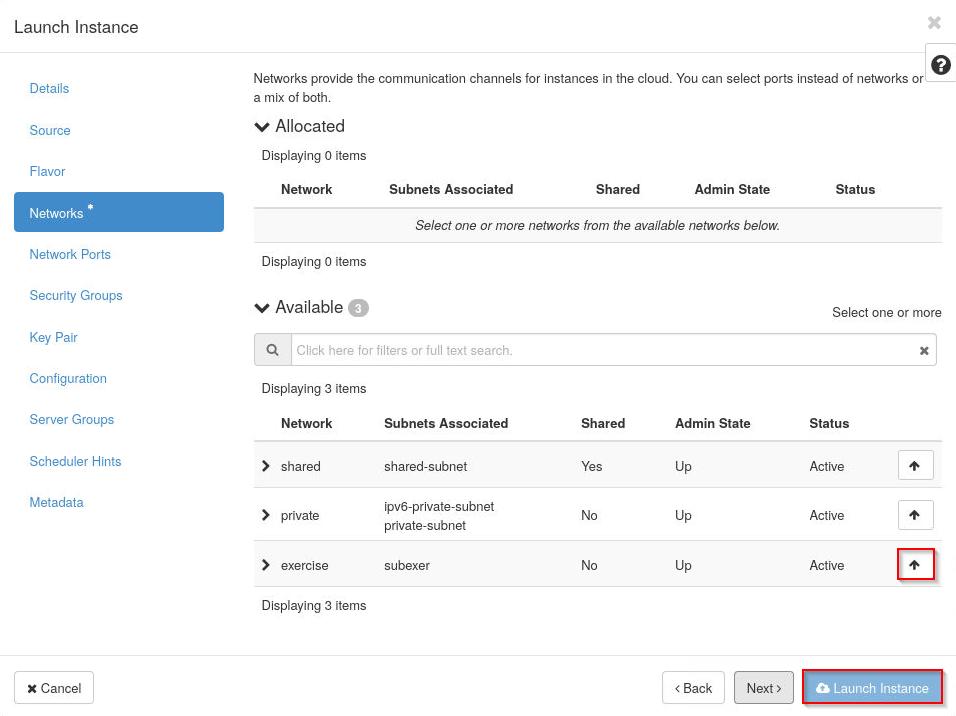
\includegraphics[width=\linewidth]{images/part4/step6.png}
    \end{center}

    \begin{stopbox}{}
        Verify that \textbf{exercise} appears under the \textit{Allocated} section. Wait for the instance to have a
        power state of \textbf{Running} before proceeding further.
    \end{stopbox}

    \item Log out of the \textit{Horizon Dashboard} and close the web browser.
    
    \item If a terminal window is not already open, open one and source the \textbf{\texttildemid/keystonerc-admin} file
    to load the \textbf{admin} user credentials.

    \item List the available instances and see that the instance created from the \textit{Horizon Dashboard} appears.
\begin{lstlisting}
ubuntu@workstation:~$ openstack server list
\end{lstlisting}

    \begin{center}
        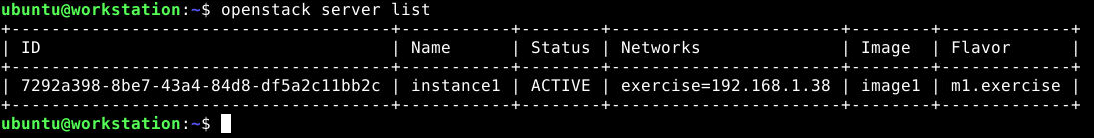
\includegraphics[width=\linewidth]{images/part4/step9.png}
    \end{center}

    \item Delete the \textbf{instance1} instance.
\begin{lstlisting}
ubuntu@workstation:~$ openstack server delete instance1
\end{lstlisting}

    \begin{center}
        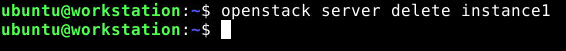
\includegraphics[width=\linewidth]{images/part4/step10.png}
    \end{center}

    \item List the instances again to verify that \textbf{instance1} was deleted successfully.
\begin{lstlisting}
ubuntu@workstation:~$ openstack server list
\end{lstlisting}

    \begin{center}
        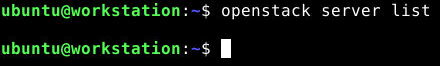
\includegraphics[width=\linewidth]{images/part4/step11.png}
    \end{center}

    \item Create a new instance named \textbf{instance2}. Use the previously created \textbf{image2} image,
    \textbf{m1.exercise} flavor, and \textbf{exercise} network.
\begin{lstlisting}
ubuntu@workstation:~$ openstack server create \
> --image image2 \
> --flavor m1.exercise \
> --nic net-id=exercise \
> --wait instance2
\end{lstlisting}

    \begin{center}
        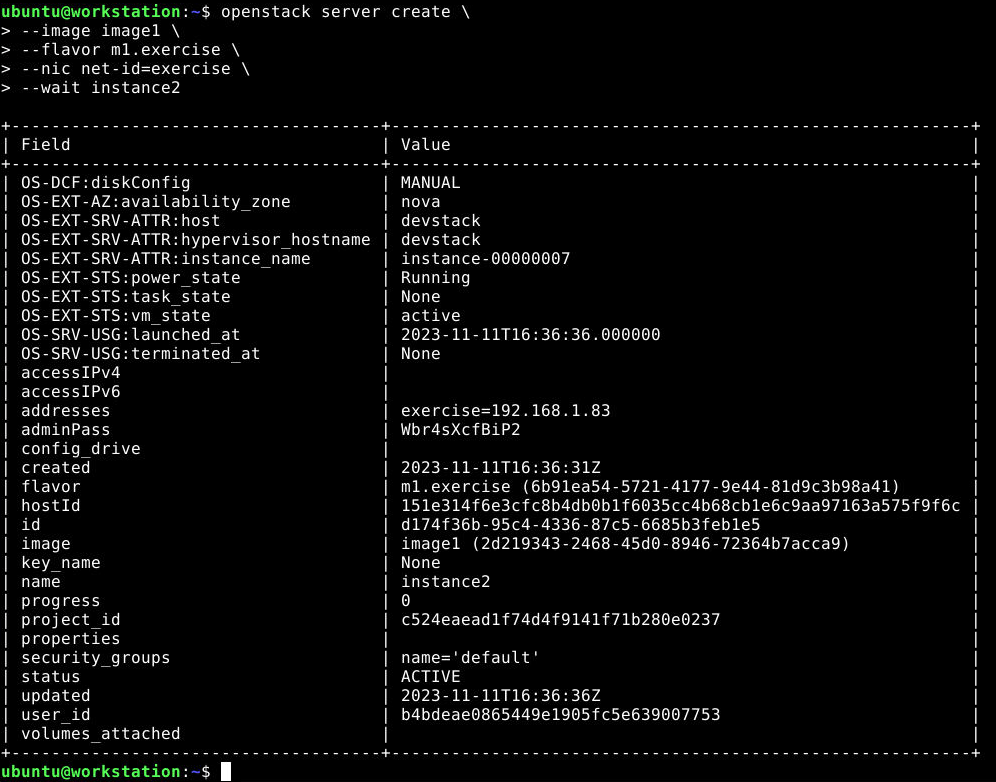
\includegraphics[width=\linewidth]{images/part4/step12.png}
    \end{center}

    \item List all the available instance to verify that the \textbf{instance2} instance is running.
\begin{lstlisting}
ubuntu@workstation:~$ openstack server list
\end{lstlisting}

    \begin{center}
        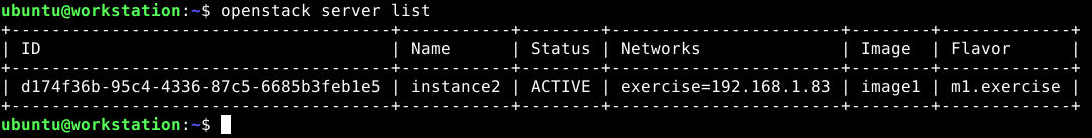
\includegraphics[width=\linewidth]{images/part4/step13.png}
    \end{center}

    \item Leave the terminal window open and continue to the next task.

\end{enumerate}

\section{Verifying the Functionality of an Internal Instance}
\label{sec:verifying_the_functionality_of_an_internal_instance}
In this task, you will connect to the instance and verify the flavor settings. You will also pause and stop an isntance
using the \textit{OpenStack Unified CLI}.

\begin{enumerate}
    \item If a terminal window is not already open, open one and source the \textbf{\texttildemid/keystonerc-admin} file
    to load the \textbf{admin} user credentials.

    \item List all the available instances to find the name of the running instance.
\begin{lstlisting}
ubuntu@workstation:~$ openstack server list
\end{lstlisting}

    \begin{center}
        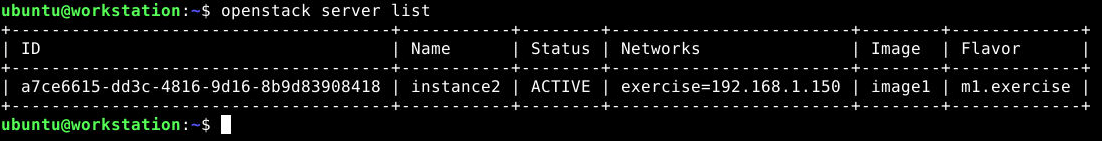
\includegraphics[width=\linewidth]{images/part5/step2.png}
    \end{center}

    \item Access the instance's details to retrieve its flavor.
\begin{lstlisting}
ubuntu@workstation:~$ openstack server show instance2
\end{lstlisting}

    \begin{center}
        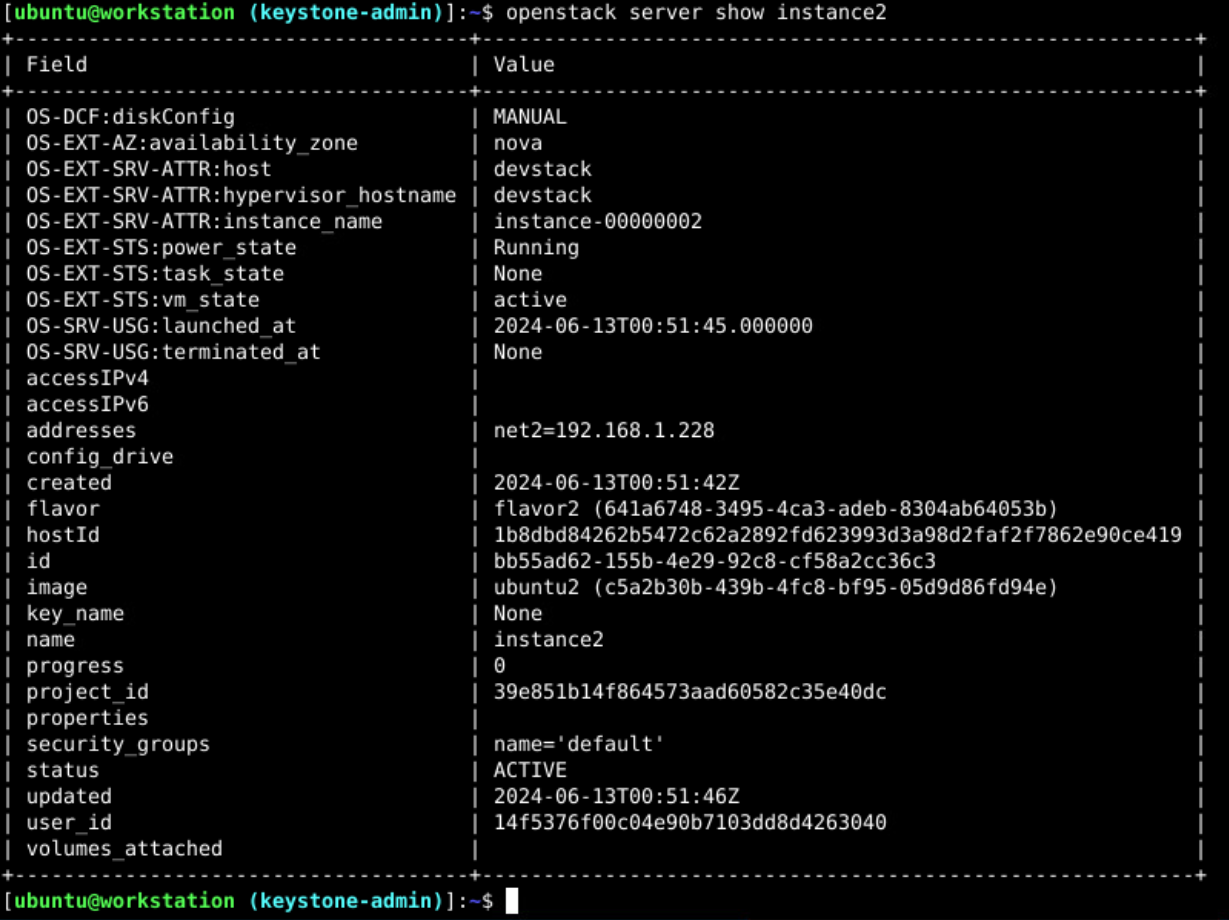
\includegraphics[width=\linewidth]{images/part5/step3.png}
    \end{center}

    \item Review the specifications of the \textbf{m1.exercise} flavor.
\begin{lstlisting}
ubuntu@workstation:~$ openstack flavor show m1.exercise
\end{lstlisting}

    \begin{center}
        \includegraphics[width=\linewidth]{images/part5/step4.png}
    \end{center}

    \item Retrieve the URL for the noVNC console connection. Right click the link and select \textbf{Open Link}.
\begin{lstlisting}
ubuntu@workstation:~$ openstack console url show \
> instance2 | grep http
\end{lstlisting}

    \begin{center}
        \includegraphics[width=\linewidth]{images/part5/step5.png}
    \end{center}

    \item Log in to the \textbf{instance2} instance as \textbf{root} with the password \textbf{secret}.
    
    \item Use the \textbf{\texttt{free}} command to ensure that the RAM and swap amount matches the one defined by the
    flavor, which is \textbf{1024 MB}.
\begin{lstlisting}
root@instance2:~# free
\end{lstlisting}

    \begin{center}
        \includegraphics[width=\linewidth]{images/part5/step7.png}
    \end{center}

    \item Use the \textbf{\texttt{df}} command to ensure that the instance has a disk size of \textbf{10 GB}, as defined
    by the flavor.
\begin{lstlisting}
root@instance2:~# df -h
\end{lstlisting}

    \begin{center}
        \includegraphics[width=\linewidth]{images/part5/step8.png}
    \end{center}

    \item Determine the number of CPUs that the instance is using. Ensure the number matches the number of VCPUs defined
    by the flavor, which is \textbf{1}.
\begin{lstlisting}
root@instance2:~# lscpu
\end{lstlisting}

    \begin{center}
        \includegraphics[width=\linewidth]{images/part5/step9.png}
    \end{center}

    \item Use the \textbf{\texttt{ping}} command from the instance to reach the DHCP server defined for the network.
    Leave the \textbf{\texttt{ping}} command running, as it will be used in the following steps.
\begin{lstlisting}
root@instance2:~$ ping 192.168.1.2
\end{lstlisting}

    \begin{center}
        \includegraphics[width=\linewidth]{images/part5/step10.png}
    \end{center}

    \item While the \textbf{\texttt{ping}} command is active, switch back to the terminal on \textbf{workstation}. Use
    the command below to pause \textbf{instance2}.
\begin{lstlisting}
ubuntu@workstation:~$ openstack server pause instance2
\end{lstlisting}

    \begin{center}
        \includegraphics[width=\linewidth]{images/part5/step11.png}
    \end{center}

    \item Switch back to the console of \textbf{instance2} and observe the behavior of the instance.

    \begin{notebox}{}
        Notice that the instance is paused and that the \textbf{\texttt{ping}} command are no longer going through.
    \end{notebox}

    \item Switch back to the terminal on \textbf{workstation}. Use the command below to unpause \textbf{instance2}.
\begin{lstlisting}
ubuntu@workstation:~$ openstack server unpause instance2
\end{lstlisting}

    \begin{center}
        \includegraphics[width=\linewidth]{images/part5/step13.png}
    \end{center}

    \item Switch back to the console of \textbf{instance2} and observe the behavior of the instance.
    
    \begin{notebox}{}
        Notice that the instance is unpaused and that the \textbf{\texttt{ping}} commands are continuing.
    \end{notebox}

    \item Switch back to the terminal on \textbf{workstation}. Use the command below to stop \textbf{instance2}.
\begin{lstlisting}
ubuntu@workstation:~$ openstack server stop instance2
\end{lstlisting}

    \begin{center}
        \includegraphics[width=\linewidth]{images/part5/step15.png}
    \end{center}

    \item Switch back to the console of \textbf{instance2} and observe the behavior of the instance.
    
    \begin{notebox}{}
        Notice that the console to the instance is no longer available.        
    \end{notebox}

    \item Switch back to the terminal on \textbf{workstation}. Start \textbf{instance2}.
\begin{lstlisting}
ubuntu@workstation:~$ openstack server start instance2
\end{lstlisting}

    \begin{center}
        \includegraphics[width=\linewidth]{images/part5/step17.png}
    \end{center}

    \item List all instances and check the status of \textbf{instance2}.
\begin{lstlisting}
ubuntu@workstation:~$ openstack server list
\end{lstlisting}

    \begin{center}
        \includegraphics[width=\linewidth]{images/part5/step18.png}
    \end{center}

    \item Delete \textbf{instance2}.
\begin{lstlisting}
ubuntu@workstation:~$ openstack server delete instance2
\end{lstlisting}

    \begin{center}
        \includegraphics[width=\linewidth]{images/part5/step19.png}
    \end{center}

    \item List all available instances to verify the \textbf{instance2} instance has been deleted.
\begin{lstlisting}
ubuntu@workstation:~$ openstack server list
\end{lstlisting}

    \begin{center}
        \includegraphics[width=\linewidth]{images/part5/step20.png}
    \end{center}

    \item Close the terminal window and the web browser.
    
    \item The lab is now complete.

\end{enumerate}

\end{document}
